%!TEX program=pdflatex
\documentclass[8pt,xcolor={dvipsnames,table,xcdraw},handout]{beamer} % option aspectratio=169 for wide screen
\usetheme[
%%% options passed to the outer theme
    progressstyle=movCircCnt,   %either fixedCircCnt, movCircCnt, or corner
    rotationcw,          % change the rotation direction from counter-clockwise to clockwise
%    shownavsym          % show the navigation symbols
  ]{AAUsimple}
  
\usepackage[utf8]{inputenc}
\usepackage{csquotes}
\usepackage[english]{babel}
\usepackage[T1]{fontenc}
\usepackage{epigraph}
\usepackage{amsmath}
\usepackage{stmaryrd}
\usepackage[ruled]{algorithm2e}
\usepackage{caption}
\usepackage[absolute,overlay]{textpos}
\usepackage{hyperref}
\SetAlCapFnt{\small}
\SetAlCapNameFnt{\small}

\setbeamerfont{caption}{size=\scriptsize}
% colored hyperlinks
\newcommand{\chref}[2]{%
  \href{#1}{{\usebeamercolor[bg]{AAUsimple}#2}}%
}
\definecolor{colorAzulBienBonito}{RGB}{0,200,255}
\newcommand{\markdone}{\textcolor{PineGreen}{$\bullet$}}
\newcommand{\markonprogress}{\textcolor{colorAzulBienBonito}{$\bullet$}}
\newcommand{\markoff}{\textcolor{PineGreen}{$\circ$}}

\usepackage{booktabs}
\usepackage{makecell}
\usepackage{multicol}
\usepackage{multirow}
\usepackage{PTSans}
%\usepackage[sfdefault,condensed]{roboto}
% \usepackage[sfdefault,condensed]{cabin} % This requires the font a little bit larger
\usepackage[sfdefault,condensed]{roboto}

% \usepackage{array}
% \newcolumntype{L}[1]{>{\raggedright\let\newline\\\arraybackslash\hspace{0pt}}m{#1}}
% \newcolumntype{C}[1]{>{\centering\let\newline\\\arraybackslash\hspace{0pt}}m{#1}}
% \newcolumntype{R}[1]{>{\raggedleft\let\newline\\\arraybackslash\hspace{0pt}}m{#1}}


\title[Smart usage of context information for the analysis, design and generation of power-aware policies for MSAs]{Smart usage of context information for the analysis, design and generation of power-aware policies for mobile sensing apps}
         
\author[Cinvestav-Tamaulipas]{Rafael Pérez Torres}

\institute[
  ITL Information Technology Laboratory\\
  Cinvestav\\
  Tamaulipas
] 
{Dr. César Torres Huitzil\\Dr. Hiram Galeana Zapién}

\date{Doctoral seminar, 2017}

% specify a logo on the titlepage (you can specify additional logos an include them in institute command below
\pgfdeclareimage[height=1.5cm]{titlepagelogo}{cinvestav-logo/cinvestav-art-logo} % placed on the title page
\titlegraphic{\pgfuseimage{titlepagelogo}}

\setbeamersize{text margin left=5mm,text margin right=5mm} 
\graphicspath{ {images/} }

\begin{document}
% the titlepage
{\aauwavesbg%
\begin{frame}[plain,noframenumbering] % the plain option removes the header from the title page
  \titlepage
\end{frame}}

\begin{frame}{Agenda}{}
  \tableofcontents[hideallsubsections]
  %\tableofcontents
\end{frame}

%!TEX root = ../slides.tex
\section{Introduction}
\subsection{Motivation}
\begin{frame}{Research background}{Motivation}
\begin{figure}[tb]
  \centering
  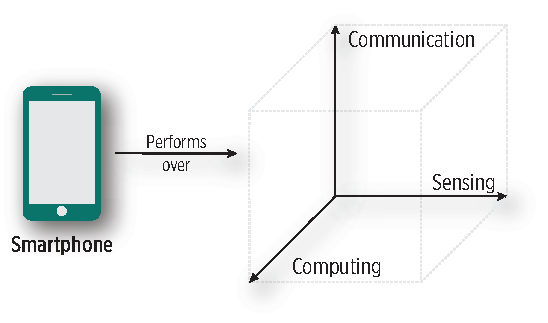
\includegraphics[width=0.4\textwidth]{vectors/smartphone-dimensions-v2}
  \caption{The advances in the communication, computing and sensing dimensions of mobile devices contribute to their acceptance by society~\cite{Islam2014}.}  
\end{figure}

\begin{block}{\small \textbf{Motivation}}
{
  \small
\begin{itemize}
  \item The sensing dimension enables \emph{context-awareness} in mobile devices, such as the smartphone.
  \item Battery advances are slower than those of other smartphone components~\cite{Kjaergaard2012}, growing 5-10\% yearly~\cite{Ma2012,Evarts2015}, a critical issue for the \textbf{mobile sensing applications}.
  % \item Battery advances are slower than those of other smartphone components~\cite{Kjaergaard2012}, growing 5-10\% yearly~\cite{Ma2012,Evarts2015}.
  % \item The energy constraint is critical for the continuous access to sensors required by \textbf{mobile sensing applications}. 
  \item Scientific efforts have been done for achieving the energy efficiency of the GPS location provider.
  \item The understanding of mobility could augment the location-awareness of the smartphone for many purposes, such as energy savings and the development of Mobility Based Services (MBSs).
  % \item As a high level of abstraction, mobility can be characterized as a sequence of frequently visited places (stay points).
\end{itemize}
}
\end{block}
\end{frame}

% \begin{frame}{Research background}{Motivation}
% \begin{block}{\small \textbf{Motivation}}
% {
%   \small
%    \begin{itemize}
%      \item For the sensing dimension, scientific efforts have been done for achieving the energy efficiency of the GPS location provider.
%      \item The understanding of mobility could augment the location-awareness of the smartphone for many purposes, such as energy savings and the development of Mobility Based Services (MBSs).
%      \item As a high level of abstraction, mobility can be characterized as a sequence of frequently visited places (a.k.a. stay points).
% \end{itemize}
% }
% \end{block}
% \end{frame}

\subsection{Research background}
%\subsection{Problem statement}
\begin{frame}{Research background}{Problem statement}
\small
\vspace{-0.5cm}
\begin{itemize}
  \item The understanding of mobility is possible at different spatial-temporal scales:
\end{itemize}

\begin{exampleblock}{\small \textbf{Fine-grain mobility patterns identification}}
 \begin{itemize}
    \item They refer to the transportation mode employed by user when moving between stay points.
    \item Given a set of values $\mathcal{V} = v_{acc~1},v_{acc~2},\ldots,v_{acc~n}$ obtained from accelerometer in the time interval $[t_1,t_2]$, identify fine-grain mobility information:
\begin{equation*}
  \text{\textbf{FineGrainMobilityIdentifier}}(\mathcal{V}) \rightarrow p_S \in \{ \text{static, walking, biking, vehicle} \}
\end{equation*}
with each $v_{acc~i} \in \mathcal{V}$ composed as $\langle acc_x,acc_y,acc_z,t \rangle$.
  \end{itemize} 
\end{exampleblock}

\begin{exampleblock}{\small \textbf{Coarse-grain mobility patterns identification}}
 \begin{itemize}
   \item They refer to motion at a large spatial scale related to user visiting stay points.
   \item \sloppy Given a set of values $\mathcal{V} = v_{gps~1},v_{gps~2},\ldots,v_{gps~n}$ obtained from GPS location provider in time interval $[t_1,t_2]$, identify coarse-grain mobility information:
\begin{equation*}
    \text{\textbf{CoarseGrainMobilityIdentifier}}(\mathcal{V}) \rightarrow p_S \in \{ \text{new stay point, arrival, departure} \}
\end{equation*}
with each $v_{gps~i} \in \mathcal{V}$ composed associated $\langle lat, lon, t \rangle$.
 \end{itemize}
\end{exampleblock}
\end{frame}


\begin{frame}{Research background}{Problem statement}
\small

\begin{exampleblock}{\small \textbf{Sensors sampling adaptation}}
\begin{itemize}
\item Given a set of coarse and fine-grain mobility patterns $\mathcal{P} = \{ p_{S_1}, p_{S_2}, \ldots, p_{S_n} \}$, and accuracy requirements of mobile app $req_{accuracy}$, implement a sampling policy for the adaptive duty cycling of sensors while reducing energy consumption:
\begin{equation*}
  \text{\textbf{PolicyGeneration}}( \mathcal{P}, req_{accuracy}) \longrightarrow{} \mathcal{S}_{conf}
\end{equation*}
where $\mathcal{S}_{conf} \rightarrow s, \mathcal{T}_{real}$ represents the sampling $\mathcal{T}_{real}$ that must be implemented for sensor $s$.
The $req_{accuracy}$ refers to the granularity of GPS sampling.
\end{itemize}
\end{exampleblock}

\begin{figure}[tb]
  \centering
  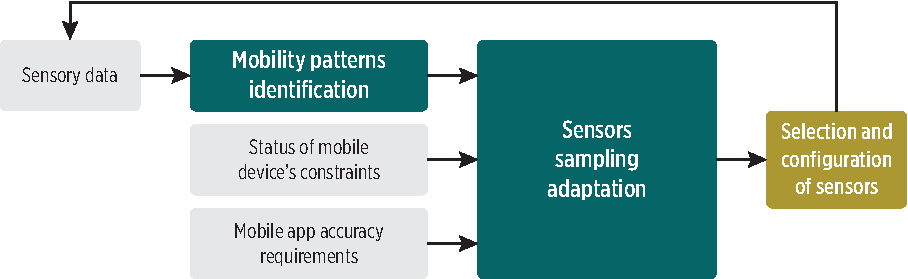
\includegraphics[width=0.7\textwidth]{vectors/problems-incorporation-v2}
  \caption{Interaction between problems.}
\end{figure}
\end{frame}

% \subsection{Hypothesis}
\begin{frame}{Research background}{Hypothesis}
\small
\begin{block}{\small \textbf{Hypothesis}}
\renewcommand{\baselinestretch}{1.4}
\begin{itemize}
  \item The energy consumption of continuous and extended location tracking could be reduced by means of a cognitive dynamic system that learns an expanded spatial-time model from mobility events detected from sensors data and that employs such model in a cognitive controller for dynamically adapting GPS sampling rate through sampling policies tailored to current mobility state.
\end{itemize}
\end{block}
\end{frame}


% \subsection{Objectives}
\begin{frame}{Research background}{Objectives}
\small
\begin{block}{\small \textbf{Main objective}}
\begin{itemize}
  \item To reduce the energy consumption of mobile sensing apps, which perform continuous sensor sampling, through self-adapting power-aware policies generated from context information obtained from sensors data.
\end{itemize}
\end{block}

\begin{block}{\small \textbf{Particular objectives}}
\begin{itemize}
  \item To detect mobility patterns from context information obtained from an inertial sensor (accelerometer) and location provider (GPS).
  \item To generate an accurate representation of detected patterns for summarizing user mobility.
  \item To dynamically adapt GPS sampling rate by means of a cognitive controller that employs the learned mobility representation and accuracy requirements for implementing power-aware sampling policies.
  \item To ease the development of mobile sensing applications that require user location tracking, i.e., LBSs and MBSs, isolating the complexity of sensors access and the associated efficient energy management.
\end{itemize}
\end{block}
\end{frame}



% \subsection{Methodology}
\begin{frame}{Research background}{Methodology}
\small
\begin{block}{\small \textbf{Methodology}}
\begin{enumerate}
  \item \textbf{Revision of state of the art power-aware sensing techniques.}
  \item \textbf{Formal definition and selection of mobility patterns to be identified.}
  \item \textbf{Research on algorithms for detecting mobility patterns.}
  \item \textbf{Design of the \emph{Mobility Events Detector}.}
  \item \textbf{Design of adaptive policies for energy efficient usage of sensors.}
  \item \textbf{Design of the Cognitive Controller.}
  \item \textbf{Development of a middleware involving the \emph{Mobility Events Detector} and the Cognitive Controller for the Android platform.}
  \item Experimentation in terms of spatial-time accuracy and energy efficiency.
\end{enumerate}
\end{block}
\end{frame}

%!TEX root = ../slides.tex
\section{State of the art}
\subsection{Mobile Sensing Apps}
\begin{frame}{State of the art}{Taxonomy of solutions}
\begin{figure}
  \centering
  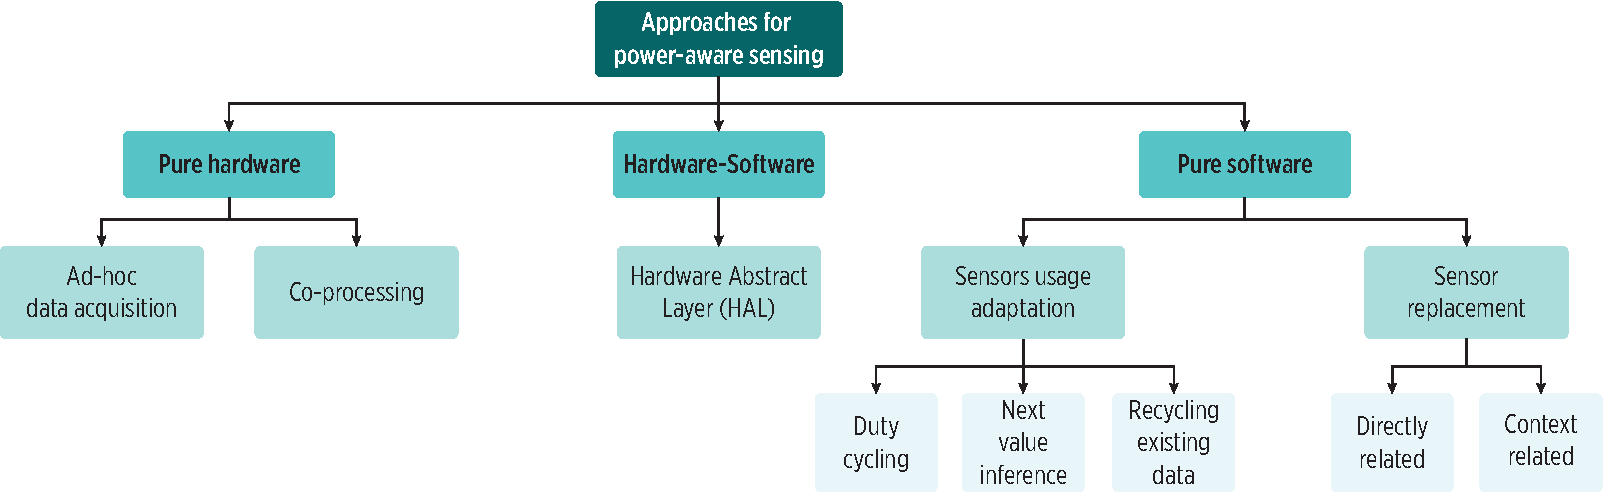
\includegraphics[width=0.9\textwidth]{vectors/approaches-taxonomy-for-slides}
  \caption{Taxonomy of solutions for power-aware sensing in mobility sensing systems.}
\end{figure}
\end{frame}

\subsection{Remarks}
\begin{frame}{State of the art}{Remarks}
\small
\begin{block}{\small \textbf{Remarks}}
\begin{itemize}
  \item The exploitation of coarse and fine-grain mobility information for modeling and characterizing user mobility has been barely explored.
  \item Although some of the proposed solutions employ a duty cycling strategy, it is fixed and obeys to instant mobility information, neglecting the temporal evolution of user mobility.
  \item A spatial-time accurate and energy efficient adaptive sampling could be produced by a cognitive approach that understands long-term mobility from fine and coarse-grain mobility events.
  \item The cognitive approach goes beyond typical pattern recognition and classic control strategies that follow a static configuration, as it evolves (in the learning and action tasks) across time.
  \item The smartphone itself could augment not only its location but also its mobility awareness (per-user basis).
\end{itemize}
\end{block}
\end{frame}
\section{Theoretical framework} 
\label{sec:theoretical_framework}

This section describes basic aspects about terms and elements involved in the problem statement which are also fundamental for a better comprehension of the state of art of this research.

\subsection{Context-aware computing}
\label{sub:context_aware_computing}

Since their introduction to market, mobile devices have evolved from basic cell phones and media players to complex and sophisticated devices like smartphones \cite{Charlesworth2009,Schmidt2011}.
Sensors, advanced wireless communication interfaces and other technological improvements have provided them with more features to be employed in any daily activity.

Furthermore, this set of computing elements have been responsible of the invention of the mobile computing area.
Mobile computing are those computing tasks that can be executed in portable devices while in motion, without losing their computing abilities and accessing to resources at remote locations through wireless networks.
That is, compute tasks anytime and anywhere.

After the invention of mobile computing, the notion of location and context in terms of mobility emerged. 
Location is a simple concept indicating the position of the user in a referenced system. 
The system can be such abstract as the \emph{GPS} or very specific like indoors, e. g. the cafeteria at university campus.

On the other hand, context is a broader and more generic concept.
Oxford dictionary defines concept as:
\begin{quotation}
  The circumstances that form the setting for an event, statement, or idea, and in terms of which it can be fully understood.
\end{quotation}
This definition gives an idea of its abstractness.

Regarding to mobile computing, context still being a non-fully established term.
In \cite{Bellavista2012} several definitions of context are listed:
\begin{itemize}
  \item{Context contains information addressing ``where you are, who you are with, and what resources are nearby'', [Schilit et al. 1994]}.
  \item{Context contains ``any information that can be used to characterize the situation of an entity'', [Dey and Abowd 2000]}.
  \item{Context comprises ``elements for the description of this context information [that] fall into five categories: individually, activity, location, time, and relations'', [Zimmermann et al. 2007]}.
  \item{Context is the ``set of variables that may be of interest for an agent and that influence its actions'', [Bolchini et al. 2009]}.
  \item{Context is ``a four-dimensional space composed of \emph{computing context}, \emph{physical context}, \emph{time context}, and \emph{user context}'', [Chen and Kotz 2000]}.
\end{itemize}

This research considers the latter definition along its development.


\subsection{Mobile sensing apps}
\label{sub:mobile_sensing_apps}

Current trends show there is a large set of applications on which smartphones can be used for. Most of these applications leverage the smartphones’ mobility features and their ability to sense the environment, which turn them into \emph{omni-sensors} \cite{Perez-Torres2012}.

Given the chance to perceive environment, data coming from sensors can be analyzed to detect patterns that represents information about user’s context.
The context then can be used to feedback user with information about his or her activities and adapt smartphone’s behavior accordingly.

As stated, the set of mobile apps that are able to perform tasks related to data collection from sensors and discovering information are called \emph{mobile sensing apps}.

The improvements in data analysis algorithms and similar techniques employed by mobile sensing apps locally at the smartphone and / or in the cloud are increasing the \emph{smartness} of these devices day by day.
In this way, smartphones can get involved in high level logical activities, not only in simple sensor readings or abstract data analysis tasks.

Because of this, the notion of smartphone will be upgraded to \emph{cognitive-phone} \cite{Campbell2012}.
This new class of devices will be able to understand people life patters, reason about their health and well-being and even intervene on their behalf.


\subsubsection{Stages of mobile sensing apps}
\label{sub:stages_of_mobile_sensing_apps}

The duty of mapping raw data into meaningful information for user can become quite complex.
This complexity level depends on the specific characteristics of the sensor being used and the mobile app requirements.

Although the differences in mobile apps and the sensors embedded in mobile devices, some steps are common in their internal functionality.
The list of these steps include the stages of sensor reading, an optional filtering, feature extraction, classification, and post-processing \cite{Ra2012}.
These stages can form a loop, as seen in Figure \ref{fig-mobile-sensing-apps-stages}, that powers up the mobile app.

A basic description of the stages is as follows:
\begin{itemize}
  \item \textbf{Sensor reading:} It includes the request to sensors for reading data from the environment. 
  Common tasks performed in this stage are windowing and framing.

  \item \textbf{Filtering (optional):} In this stage is possible to filter out uninterested data, like outliers or noise.
  Filling data gaps can also be done.
  The purpose of the stage is to prepare a clean and uniform set of data for its use in further steps.

  \item \textbf{Feature extraction:} It performs the extraction of features that helps to discriminate between activities in the classification stage.
  The feature extraction to be employed depends on the type of mobile app being developed.
  The features to be computed can be:
  \begin{itemize}
    \item \emph{Deterministic:} Simple deterministic transformations of raw sensor data, for example frequency content.
    \item \emph{Probabilistic:} Calculated with probability measures, for example the user likelihood of being in a certain location.
  \end{itemize}

  \item \textbf{Classification:} It involves the execution of the mobile app specific classifier.
  Because of the complexity of human activities and the noise existing in sensor data, the classification algorithm are almost always probabilistic, although machine learning techniques have also been used \cite{Choudhury2008}.
  The classifiers can make use of user’s context to improve their performance.

  This stage is the most power consuming one and the execution time may take from seconds up to hours, depending on the data being classified (e. g. in the case of human behavior recognition).
  Because of this, the classifier can be executed locally at the smartphone or in external elements like the cloud.

  \item \textbf{Post-processing:} The classification of data may trigger another loop of continuous sensing-compute chain or other mobile app specific tasks such as displaying feedback to the user or initiating network communication.

\end{itemize}

\begin{figure}
\centering
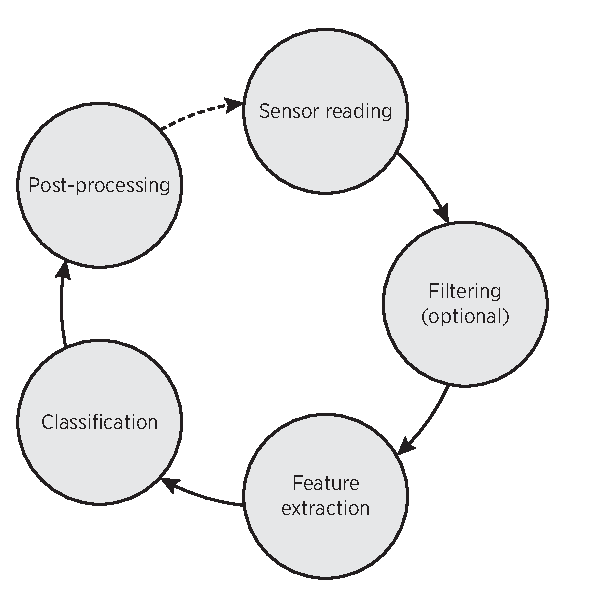
\includegraphics[scale=0.6]{msa-stages}
\caption[Common stages of mobile sensing apps]{Common stages of mobile sensing apps.}
\label{fig-mobile-sensing-apps-stages}
\end{figure}

\subsubsection{Sensing scale of mobile sensing apps}\label{sub:sensing-scale-of-msa}

Depending on the purpose of the mobile app, it may be required to obtain data from one or more users.
The target audience size of the mobile app is known as the \emph{sensing scale}.
There are two sensing scales:
\begin{itemize}
  \item \textbf{Individual sensing scale:} Involves collecting and analyzing data coming from a single person.
  Typically, data refer to track user’s exercise routine and the information is not shared.

  \item \textbf{Community sensing scale:} Involves collecting and analyzing data coming from several users who share a common goal.
  It needs to respond to user specific needs of privacy and anonymity.
  
  This sensing scale is often referred as mobile crowd-sensing and classic examples include traffic monitoring, detection of available parking slots, etc.

  An implicit detail in this sensing scale is the need of a centralized node that acts as a sink of data where analysis processes are executed.
\end{itemize}

This research is conducted targeting the individual sensing scale since the policies to be generated consider analysis of data coming from a single person.


\subsubsection{Paradigms of mobile sensing apps}\label{sub:paradigms-of-msa}

The way how sensors are employed and whether explicit user input is required by a mobile app is known as the \emph{mobile sensing paradigm} \cite{Lane2010}.

There are two sensing paradigms:
\begin{itemize}
  \item \textbf{Opportunistic:} It aims automatic data collection without human participation at all. A remarkable issue of this paradigm is determining the best moment to perform a sensor reading.

  \item \textbf{Participatory:} It leverages the abilities of people requiring their participation to describe the data and to decide the best moment for their capture.

  However, this human dependence can also be a source of errors and noisy data since user is able to upload mislabeled data or even to not to have participation at all.
\end{itemize}


This research is conducted by following the opportunistic paradigm since the smart policies to be generated will decide the duty cycle that sensors must observe, avoiding user participation.


\subsection{Mobile sensing apps examples}
\label{sub:mobile_sensing_apps_examples}

Mobile sensing apps have evolved from apps with specific sensor usage, like using the accelerometer to change the orientation of the screen, to more complex tasks like detecting the user activity e. g. walking, running, climbing stairs, etc.
The usage possibilities offered by mobile sensing apps are high and even increasing after a new sensor is embedded in a smartphone.

In \cite{Wang2012} the \emph{WalkSafe} mobile app is described.
This app improves the safety of pedestrians that walk and talk. WalkSafe leverages the user's context employing the back camera of the smartphone to detect vehicles approaching the user, alerting her or him of a potential unsafe situation.

WalkSafe implements machine learning techniques for detecting the front and back views of moving vehicles.
It employs image recognition algorithms trained off-line with datasets of positive (pictures of front and back views of vehicles) and negative (pictures of side views of vehicles and urban environments) samples producing a set of features for building the car detection model.

Once the model is created, it is uploaded to the phone for its usage in the on-line detection process.
When a phone call is received, the smartphone takes pictures from the back camera, fixes their orientation with accelerometer data, and passed them to the detection module for their processing in real time.
If a car approaching the user is detected, then a vibrating alert is emitted.


Another example of context information usage is \emph{BeWell} \cite{Lane2011a}, which is an app that can monitor and promote some aspects of physical and emotional well-being.
BeWell continuously tracks user behavior along three health dimensions in an \emph{opportunistic} sensing way.

Classifications algorithms are run directly on the phone to infer context information about user's sleep duration, physical activity, and social interaction from sensor data.
BeWell assigns a score to these dimensions and gives a graphical feedback of them to the user.
Sleep duration is inferred by detecting the absence of movement of phone at night.
Physical activity is detected thanks to accelerometer inferring walking, stationary, or running states of the user.
Social interaction is obtained thanks to microphone samples that are used to detect speech or silence time lapses.


A final instance of mobile sensing apps, that employs a \emph{pluggable} sensor via Bluetooth, is \emph{NeuroPhone} \cite{Campbell2010}.
This app works employing neural signals obtained from an electroencephalography (EEG) headset to control smartphones.


Neurophone is a brain-controlled address book dialing app that leverages the generation of P300 \footnote{\emph{P300} is a neuroscience term that refers to a positive peak with a latency of 300 $ms$ that is elicited when brain concentrates on a task specific stimulus among a pool of stimulus.} signals in human brain.
The smartphone shows a sequence of pictures of address book contacts and a potential P300 brain is elicited when a photo matches the person whom the user wishes to call.
The data generated by the EEG headset is transmitted to the smartphone, on which a classification process detects an actual P300 and triggers the contact’s phone number dialing.

% \subsubsection{Convergence of sensing applications into the IoT}
% % Mention that smart devices are connecting people, globally and that is the final objective of them.
% Mobile sensing apps are contributing to the adoption of mobile devices by society.
% By leveraging the communication facilities (for instance, the Internet enabled feature) of smart devices, the vision of future world is one such people will be globally connected with others anywhere and anytime.

% % Mention that a fully connected world has been spotted in other scenarios.
% This vision of a fully connected world has been also chased in other scenarios, like the industry, where the items to be connected are common real world objects like tools, machines, buildings, vehicles, etc.
% % Introduce the smart objects
% Such items are enhanced with an identification mechanism like RFID and basic computation, sensing, and communication facilities that turn them into smart objects \cite{Kortuem2010}.
% % Mention that when 2+ smart objects communicate, then there is a M2M
% Thanks to these enhanced capabilities, the smart objects are able to collect data of their environment and interact with other smart objects, creating a M2M communication system.

% % Introduce the objectives of M2M
% M2M communication systems aim to go beyond the industrial environment and be the base mechanism to query and deliver data between any objects of the real world.
% Such communication should be allowed in any direction, from object A to object B and vice versa.
% Thanks to this, it will be possible to collect data from sensors of a smart object or to instruct an object to behave in a particular way, modifying its environment.

% % Mention that the sets SP-MSA and SO-M2M are similar but also present differences.
% The sets conformed by smartphone--mobile sensing apps and smart objects--M2M target different scenarios but share several features shown in Table \ref{tbl:msa-vs-m2m}.
% The only aspects they do not share are the \emph{communicates with} and application purpose.
% \emph{Communicates with} refers to the type of entity a smartphone or a smart object establish communication with.
% Typically a smart object will communicate always with other smart objects, like in any M2M communication system instance.
% On the other hand, a smartphone can communicate with other objects but also with humans.
% It means that smart devices, like the smartphone, offer several interaction ways for communicating with people while smart objects do not.

% The application purpose marks another difference between smartphones and smart objects.
% A smart object has a specific purpose: it only performs a single or a reduced set of tasks, it is not designed to execute third party apps; indeed, the concept of a mobile OS is out of its scope.
% In change, a smartphone is a general purpose item that can be employed in a wide range of applications. Smart devices include a mobile OS that makes it possible to install third party apps and expand their functionality.
% Broadly speaking, a smart device, like a smartphone, can be considered a smart object but this relationship does not apply inversely.

% \begin{table}
%   \centering
%     \scriptsize
%     \begin{tabularx}{0.70\linewidth}{ccc}
%       \toprule
%       \textbf{Feature} & \textbf{Smartphone} & \textbf{Smart object} \tabularnewline
%       \midrule
%         \textbf{Context awareness} & Yes (Through sensors) & Yes (Through sensors) \tabularnewline
%         \textbf{Communication} & Yes (Wireless) & Yes (Wired, Wireless) \tabularnewline
%         \textbf{Processor} & Yes (Multi-core) & Yes (Low power consuming) \tabularnewline
%         \textbf{Storage} & Yes (In the order of Gigabytes) & Yes (reduced size) \tabularnewline
%         \textbf{\emph{Communicates with}} & Human, other objects & Other objects (machines) \tabularnewline
%         \textbf{Purpose} & General & Specific \tabularnewline
%       \bottomrule
%     \end{tabularx}
   
%     \caption{Comparison of the characteristics of smartphones versus smart objects}
%     \label{tbl:msa-vs-m2m}
% \end{table}

% In any case, the sets smartphone--mobile sensing apps and smart objects--M2M can be abstracted as systems that interconnect \emph{things} in an evolved vision of Internet known as the IoT.
% % Tell a brief IoT interaction-flow
% In the IoT every real world object has a virtual representation and can understand its environment and role in a particular activity, trigger special actions when certain events occur and materialize these actions in both physical and virtual worlds \cite{Uckelmann2011}.
% If mobile computing has the dimension of time and place, IoT adds the new dimension of thing (see Figure \ref{fig-iot-dimensions}).
% Summarizing: IoT aims to produce a fully connected world with unlimited application systems that address any real world problem.

% \begin{figure}
% \centering
% 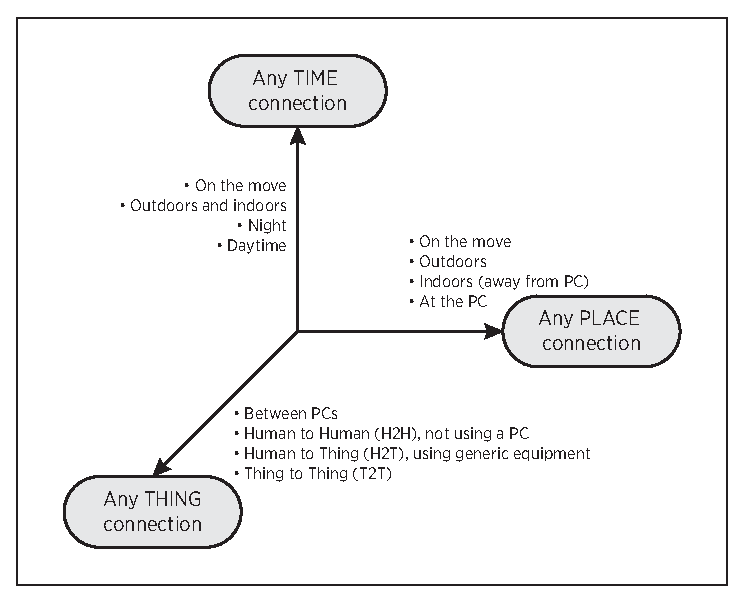
\includegraphics[scale=0.6]{iot-dimensions}
% \caption[Dimensions of the IoT]{Dimensions of the Internet of Things: time, place, thing.}
% \label{fig-iot-dimensions}
% \end{figure}
\section{Solution}
\subsection{Solution's overview}
{\aauwavesbg%
\begin{frame}[plain]
  \begin{textblock*}{8.5cm}(4.3cm,8.3cm)
  \small
  \textbf{Architecture of proposed system solution. The global perception-action cycle, the different memory types, and the internal feedback loops are observed.}
  \end{textblock*}

  \begin{textblock*}{1cm}(12cm,9.3cm)
  \scriptsize
  \insertframenumber~/~\inserttotalframenumber
  \end{textblock*}

  \centering
  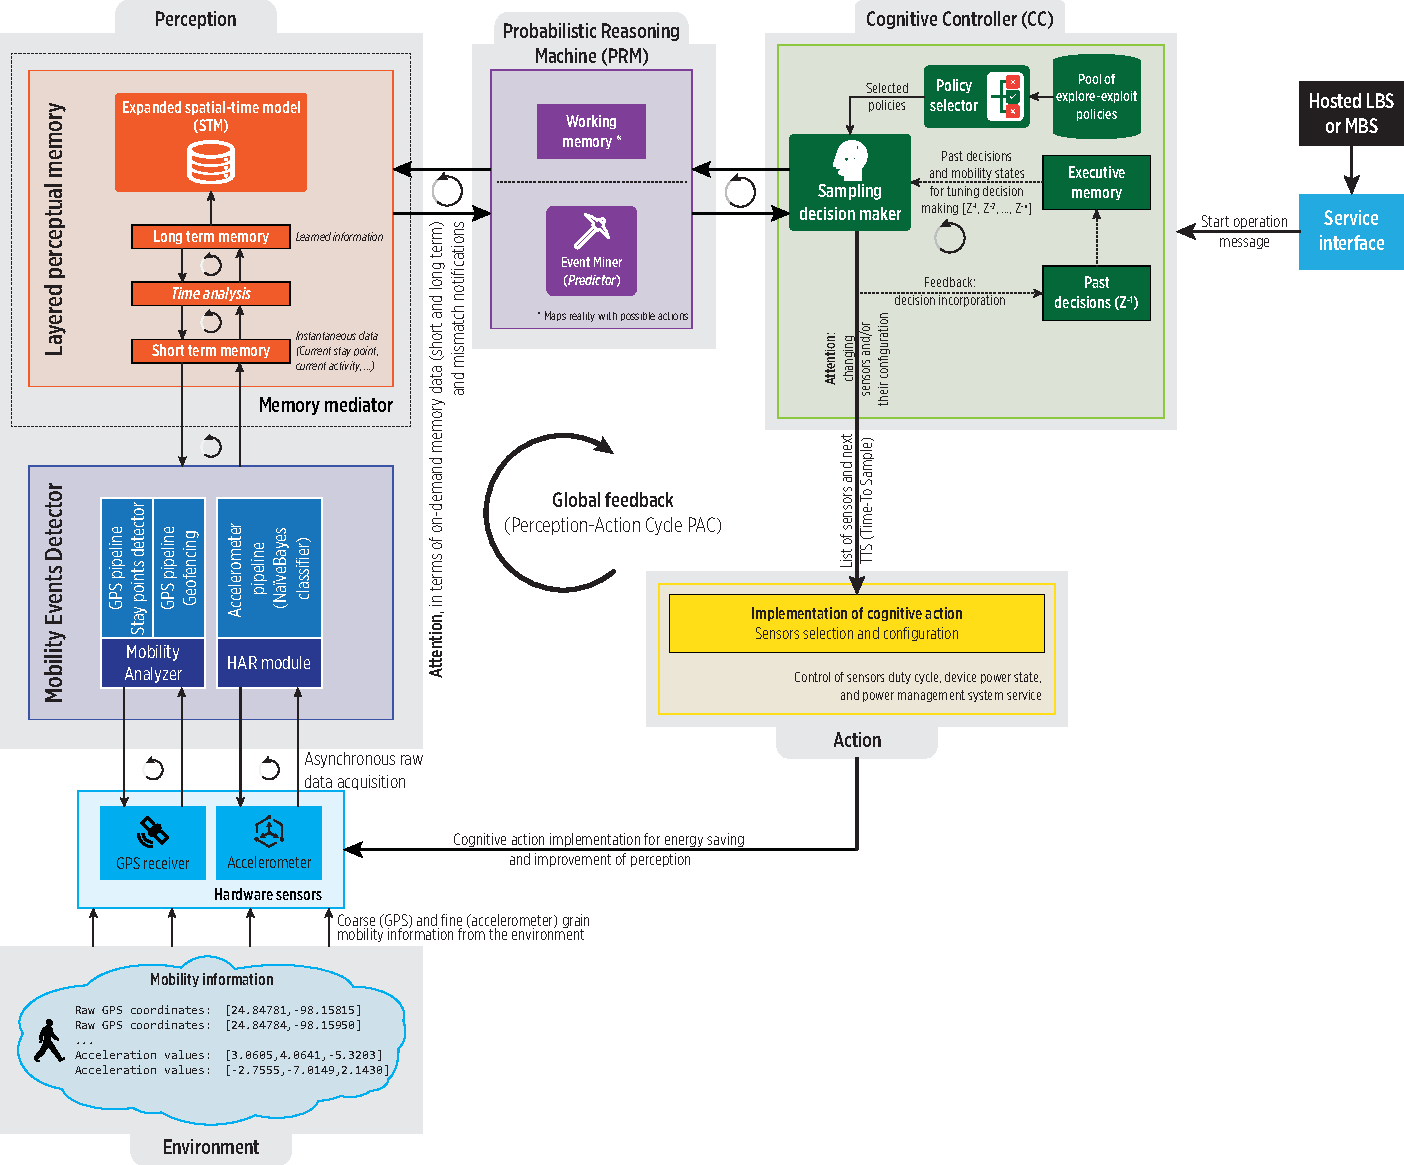
\includegraphics[width=0.98\textwidth]{vectors/inspired-cds-solution-for-slides}
  %\captionof{figure}{Architecture of proposed system solution. The global perception-action cycle and the internal loops are observed.}
\end{frame}}
%!TEX root = ../slides.tex
\section{Implementation}
%\subsection{Implementation}
\begin{frame}{Implementation}{Android device implementation}
\small

\begin{block}{\small \textbf{Smartphone device}}
The Google Nexus 6 smartphone with Android 7 was employed.
\begin{itemize}
  \item Quad-core 2.7 GHz Krait 450 mobile processor (Qualcomm Snapdragon 805 chipset).
  \item 3 GB RAM.
  \item Qualcomm Snapdragon 805 chipset.
  \item 3220 mAh battery.
\end{itemize}
\end{block}

\begin{alertblock}{\small \textbf{Technical barriers}}
\begin{enumerate}
  \item Asynchronous access to sensors, affected by sensing infrastructure (GPS satellite signal intermittency).
  \item Out-of-the-box energy saving mechanisms:
  \begin{itemize}
    \item Application specific: \textbf{App StandBy}.
    \item System wide: \textbf{Doze mode}.
  \end{itemize}
\end{enumerate}
\end{alertblock}

\begin{exampleblock}{\small \textbf{Workarounds}}
\begin{enumerate}
  \item Grace periods for sampling (\texttt{Timer} + \texttt{TimerTasks}).
  \item \texttt{Alarms}, \texttt{WakeLocks}, foreground services.
\end{enumerate}
\end{exampleblock}
\end{frame}

{\aauwavesbg%
  \begin{textblock*}{5cm}(0.3cm,0.3cm)
  \small
  \textbf{The architecture of the proposed system implemented in the Android software stack.}
  \end{textblock*}
\begin{textblock*}{1cm}(12cm,9.3cm)
  \scriptsize
  \insertframenumber~/~\inserttotalframenumber
  \end{textblock*}
\begin{frame}[plain]
  \centering
  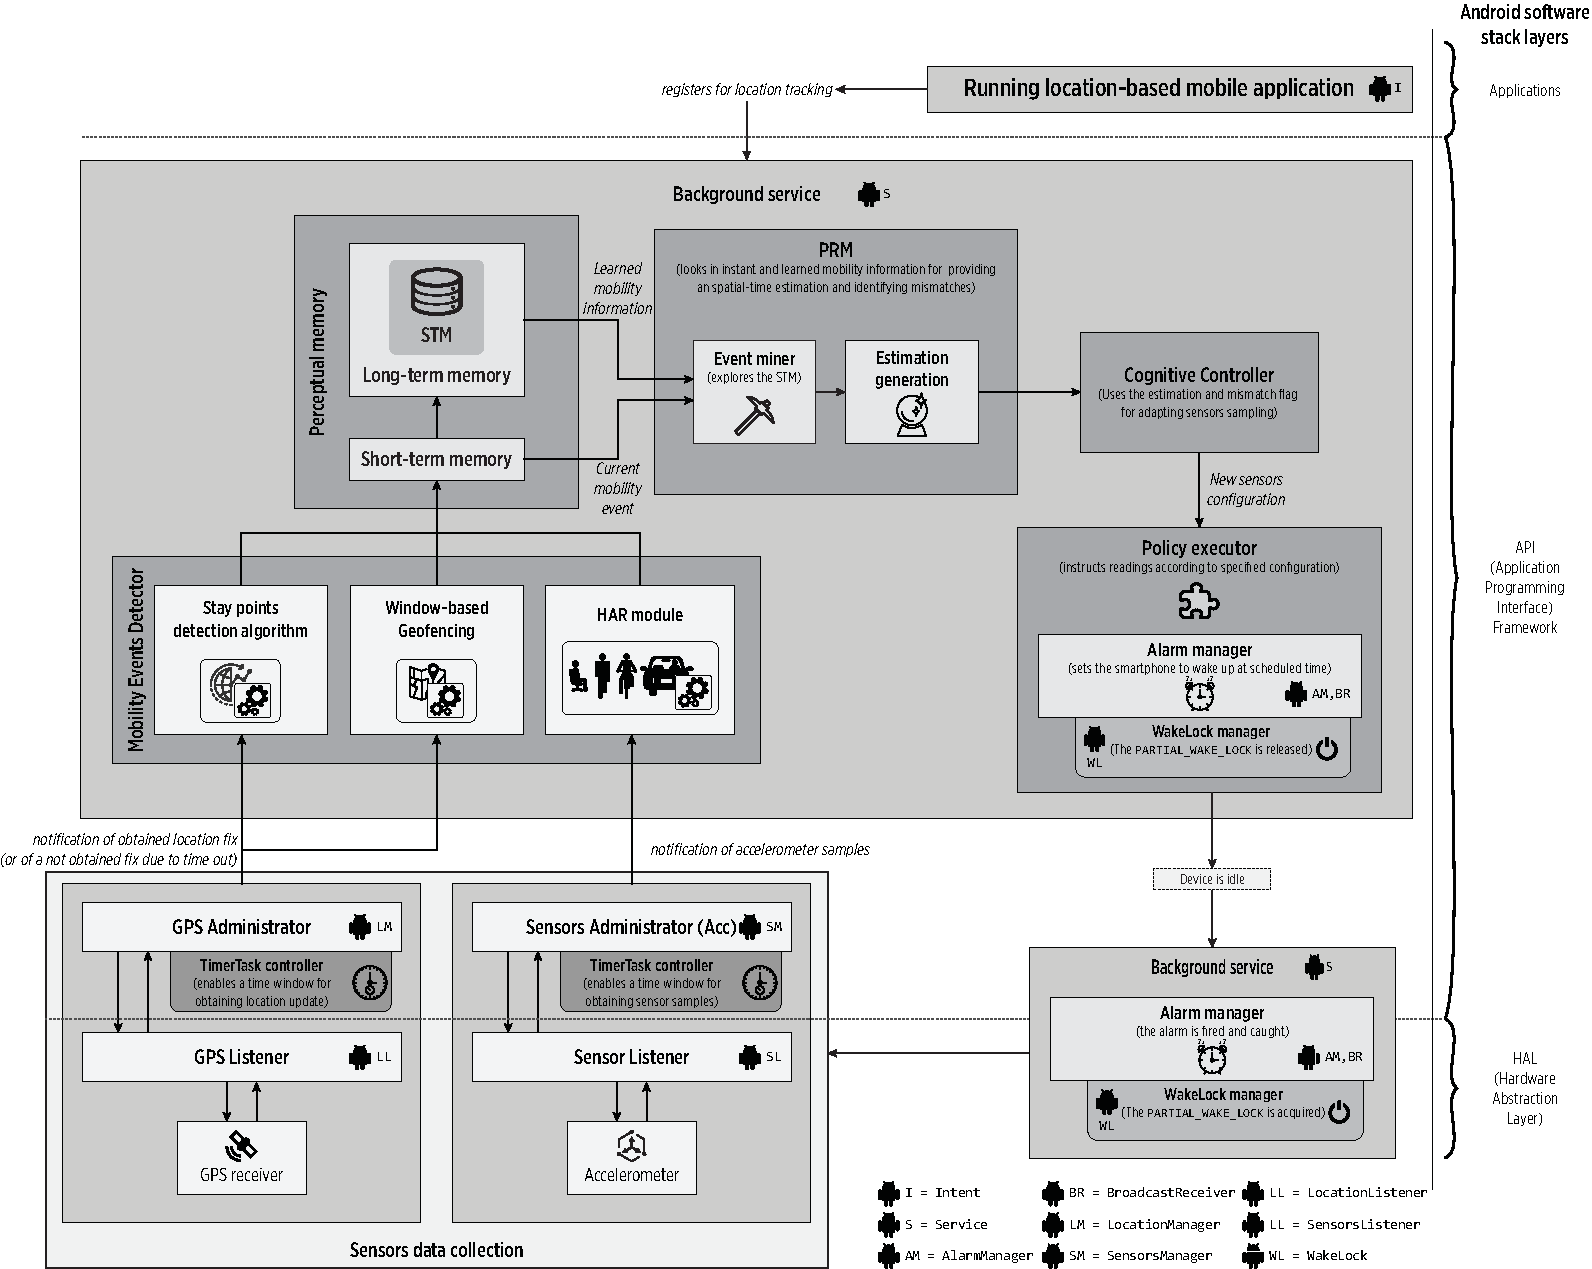
\includegraphics[width=\textwidth]{vectors/implementation}
\end{frame}}

% \begin{frame}{Implementation}{Android device implementation}
% \begin{center}
% 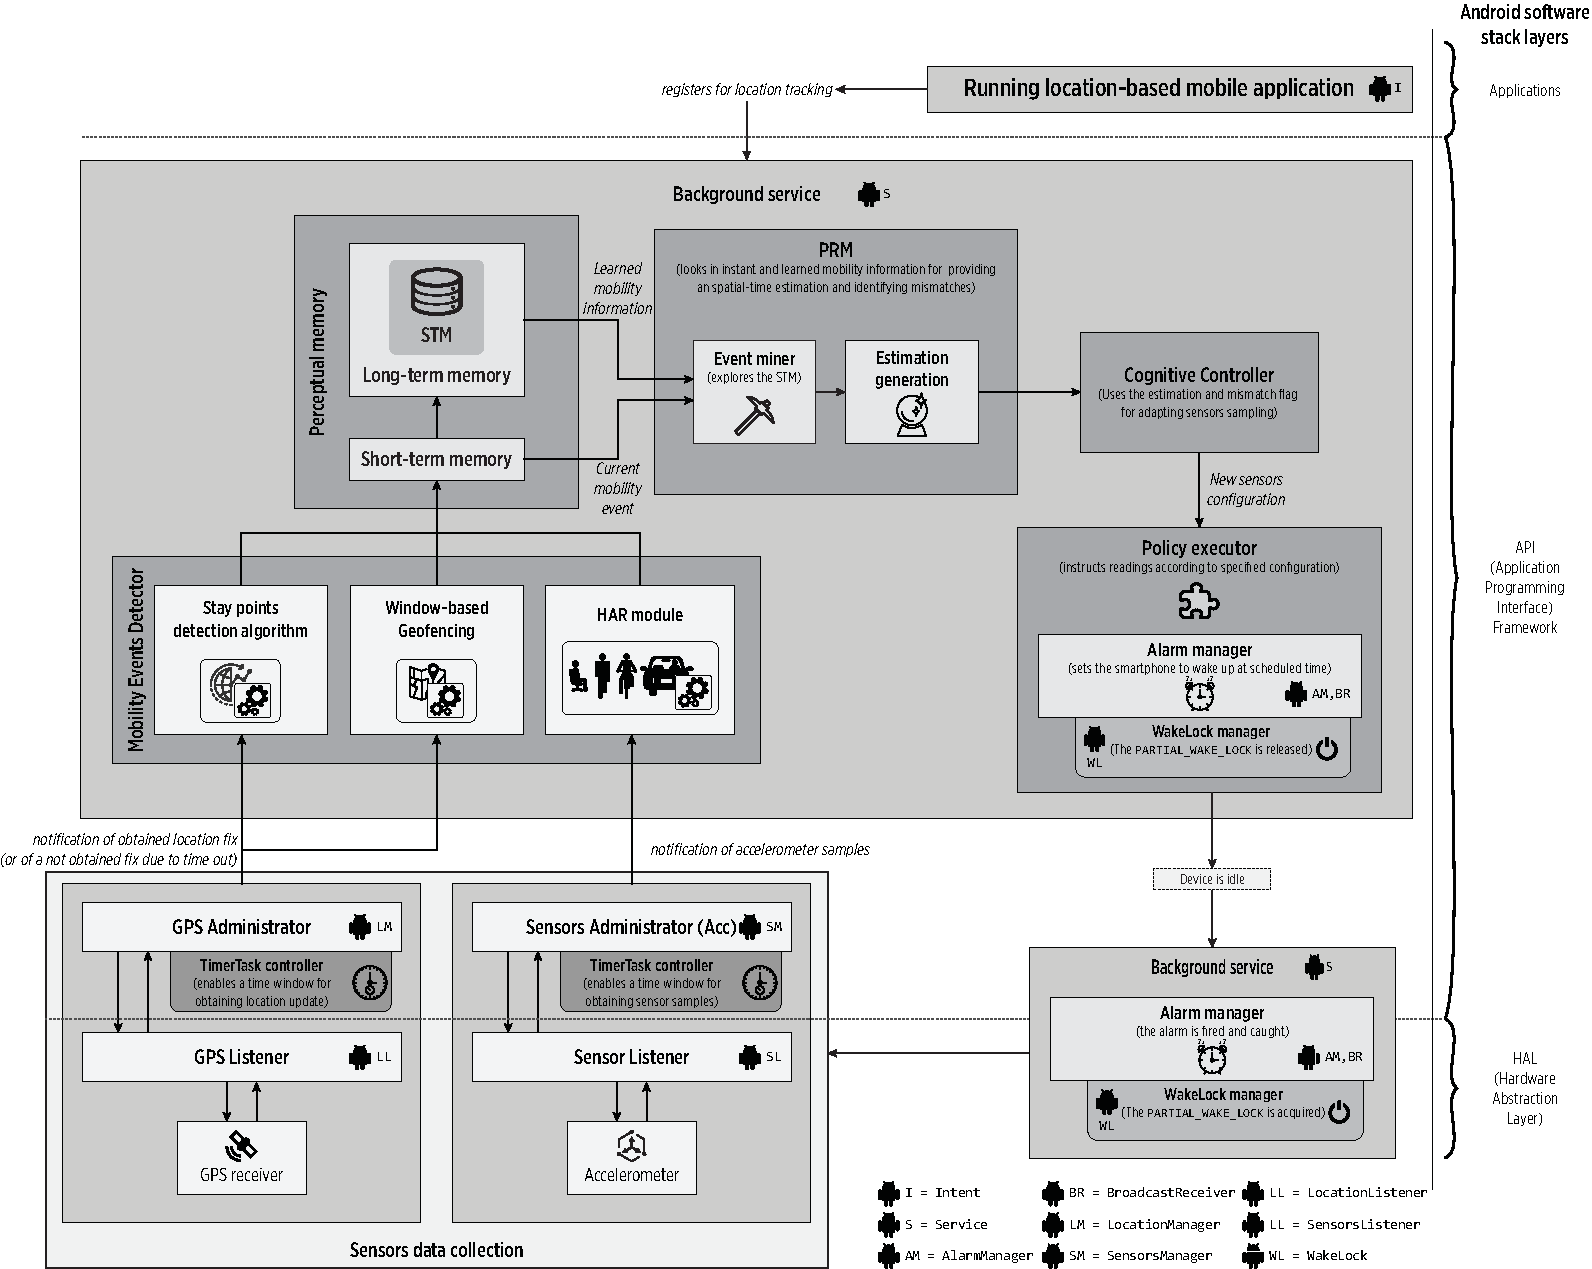
\includegraphics[width=0.8\textwidth]{vectors/implementation}
% \end{center}
% \end{frame}
%!TEX root = ../slides.tex
\section{Preliminary results}
\begin{frame}{Experimentation}{Materials and methods}
\small 
\vspace{-0.5cm}
\begin{columns}
\begin{column}[T]{0.55\textwidth}
\begin{block}{\small \textbf{Ground-truth mobility information}}
  \begin{itemize}
    \item High frequency ($1~Hz$) location data collected employing a Qstarz BT-Q1000eX GPS logger.
    \item 6 trajectories collected by the same user, mostly using a vehicle as transportation mode.
  \end{itemize}
\end{block}
\end{column}

\begin{column}[T]{0.45\textwidth}
\begin{table}
\centering
\renewcommand{\arraystretch}{0.6}
\resizebox{0.83\textwidth}{!}{%
\begin{tabular}{@{}lll@{}}
\toprule
\multirow{2}{*}{\textbf{Stay Points Detector}} & \textbf{Time threshold} ($\delta_{time}$): & $45~min$ \\
\cmidrule[0.25pt]{2-3}
 & \textbf{Distance threshold} ($\delta_{distance}$): & $500~m$ \\

\cmidrule[0.25pt]{1-3}
\multirow{3}{*}{\textbf{Geofencing}} & \textbf{Radio distance} ($gf_{distance}$): & $250~m$ \\
\cmidrule[0.25pt]{2-3}
 & \textbf{Window size} ($gf_{ws}$): & 3 \\

\cmidrule[0.25pt]{1-3}
\textbf{Sampling period}: & \multicolumn{2}{l}{1 second} \\

\bottomrule
\end{tabular}%
}
\caption{Input parameters for the discovery of ground truth mobility information.}
\label{tab:exp-gt-input-parameters}
\end{table}
\end{column}
\end{columns}

\begin{table}
\centering
\renewcommand{\arraystretch}{0.8}
\resizebox{\textwidth}{!}{%
\begin{tabular}{@{}lrrrrrr@{}}
\toprule
\multicolumn{1}{c}{\textbf{Trajectory}} & 
\multicolumn{1}{c}{\textbf{Duration (days)}} & 
\multicolumn{1}{c}{\textbf{Inside SP time (minutes)}} &
\multicolumn{1}{c}{\textbf{In traj. time (minutes)}} &
\multicolumn{1}{c}{\textbf{Total SPs}} &
\multicolumn{1}{c}{\textbf{Total visits}} &
\multicolumn{1}{c}{\textbf{Individual SP weight}} \\
\midrule


% total minutes: 7 747.17
Trajectory 1 & 5.38 & 7,442.10 (96.06\%) & 305.07 (3.94\%) & 4 & 13 &
% 12 & 
\begin{tabular}[c]{@{}rr@{}}
Home: 72.25\% & Cinvestav: 26.03\%\\ 
Bob's place: 0.94\% & Store: 0.78\%\\
\end{tabular} \\

\cmidrule{1-7}
% total minutes: 8 714.15
Trajectory 2 & 6.05 & 8,348.42 (95.80\%) & 365.73 (4.20\%) & 6 & 21 & 
% 20 & 
\begin{tabular}[c]{@{}rr@{}}
Home: 69.67\% & Cinvestav: 26.51\%\\ 
Bob's place: 1.20\% & Park: 0.99\%\\ 
Store: 0.82\% & Stadium: 0.82\%\\
\end{tabular} \\

\cmidrule{1-7}
% total minutes: 8 849.57
Trajectory 3 & 6.15 & 8,542.12 (96.53\%) & 307.45 (3.47\%) & 6 & 31 & 
% 31 & 
\begin{tabular}[c]{@{}rr@{}}
Home: 67.94\% & Cinvestav: 24.50\%\\ 
Park: 2.94\% & Bob's place: 2.58\%\\ 
Fast food: 1.15\% & City center: 0.89\%\\
\end{tabular} \\

% total minutes: 10 396.62
\cmidrule{1-7}
Trajectory 4 & 7.22 & 10,024.63 (96.42\%) & 371.98 (3.58\%) & 2 & 16 & 
% 15 & 
\begin{tabular}[c]{@{}rr@{}}
Home: 66.50\% & Cinvestav: 33.50\%\\
\end{tabular} \\

\cmidrule{1-7}
% total minutes: 10 582.42
Trajectory 5 & 7.35 & 10,026.22 (94.74\%) & 556.20 (5.26\%) & 4 & 19 & 
% 18 & 
\begin{tabular}[c]{@{}rr@{}}
Home: 67.29\% & Cinvestav: 29.33\%\\ 
Cinema: 2.41\% & City center: 0.97\%
\end{tabular} \\

\cmidrule{1-7}
Trajectory 6 & 34.31 & 47,599.62 (96.34\%) & 1,807.52 (3.66\%) & 11 & 146 & 
% 145 & 
\begin{tabular}[c]{@{}rr@{}}
Home: 65.31\% & Cinvestav: 29.36\%\\ 
Home 2: 2.81\% & Fast food: 0.71\%\\
Bob's place: 0.37\% & Restaurant: 0.36\%\\ 
Store: 0.35\% & City center: 0.30\%\\
Workshop: 0.20\% & Store 2: 0.12\%\\
Workshop 2: 0.11\%\\
\end{tabular} \\ \bottomrule
\end{tabular}%
}
\caption{Mobility information of collected ground truth trajectories (SP=stay point).}
\label{tab:ground-truth-trajectories}
\end{table}
\end{frame}


% \subsection{Stay Points Detector spatial-time accuracy}
\begin{frame}{Experimentation}{Spatial-time accuracy of \emph{Stay Points Detector} and \emph{Geofencing} modules}
\small

\begin{block}{\small \textbf{Description}}
\begin{itemize}
  \item Evaluation of the spatial-time accuracy of the \emph{Stay Points Detector} module: centroid distances and latencies.
  \item Evaluation of the spatial-time accuracy of the \emph{Geofencing} module: missed visits, and latencies.
\end{itemize}

\begin{columns}
\begin{column}[T]{0.5\textwidth}
\begin{table}
\centering
\renewcommand{\arraystretch}{0.6}
\resizebox{0.9\textwidth}{!}{%
\begin{tabular}{lll}
\toprule
\multirow{2}{*}{\textbf{Stay Points Detector}} & \textbf{Time threshold} ($\delta_{time}$): & $45~min$ \\
\cmidrule[0.25pt]{2-3}
 & \textbf{Distance threshold} ($\delta_{distance}$): & $500~m$ \\

\cmidrule[0.25pt]{1-3}
\textbf{Sampling periods}: & \multicolumn{2}{l}{30, 60, 90, 120, 150, 180 seconds.} \\

\cmidrule[0.25pt]{1-3}
\textbf{Trajectories}: & \multicolumn{2}{l}{All ground truth trajectories.} \\
\bottomrule
\end{tabular}
}
\caption{Input parameters for the spatial-time accuracy of stay points experiment.}
\end{table}
\end{column}

\begin{column}[T]{0.5\textwidth}
\begin{table}
\centering
\renewcommand{\arraystretch}{0.6}
\resizebox{0.8\textwidth}{!}{%
\begin{tabular}{lll}
\toprule
\multirow{2}{*}{\textbf{Geofencing}} & \textbf{Radio distance} ($gf_{distance}$): & $250~m$ \\
\cmidrule[0.25pt]{2-3}
 & \textbf{Window size} ($gf_{ws}$): & 3, 5, 7 \\

\cmidrule[0.25pt]{1-3}
\textbf{Sampling periods}: & \multicolumn{2}{l}{30, 60, 90, 120, 150, 180 seconds.} \\

\cmidrule[0.25pt]{1-3}
\textbf{Trajectories}: & \multicolumn{2}{l}{All ground truth trajectories.} \\

\cmidrule[0.25pt]{1-3}
\textbf{STM} & \multicolumn{2}{l}{Preloaded with ground truth stay points.} \\
\bottomrule
\end{tabular}
}
\caption{Input parameters for the spatial-time accuracy of \emph{Geofencing} experiment.}
\end{table}
\end{column}
\end{columns}
\end{block}

\begin{block}{\small \textbf{Results}}
\begin{itemize}
  \item \emph{Stay Points Detector} and \emph{Geofencing} modules performed with spatial-time accuracy:
\begin{itemize}
  \item A maximum centroid distance of $22.52~m$ is identified when employing the 180 seconds sampling period.
  \item The length of the visits missed by the \emph{Geofencing} module are under 90 seconds. Latencies are in function of the window size parameter value.
\end{itemize}
\end{itemize}
\end{block}

% \vspace{-0.5cm}
% \begin{block}{\small \textbf{Results}}
% \begin{columns}
% \begin{column}{0.65\textwidth}
% {
%   \centering
%   \includegraphics[width=0.95\textwidth]{vectors/experiments/exp-1/exp-1-centroid-distance}
% }
% \end{column}
% \begin{column}{0.3\textwidth}
% \captionof{figure}{The impact of different sampling periods on the centroid distance of identified stay points in each trajectory. A maximum centroid distance of $22.52~m$ is identified when employing the 180 seconds sampling period.}
% \end{column}
% \end{columns}

% \end{block}
\end{frame}




% \subsection{Geofencing accuracy}
% \begin{frame}{Experimentation}{\emph{Geofencing} module spatial-time accuracy: Description}
% \small 
% \vspace{-0.4cm}
% \begin{columns}
% \begin{column}[T]{0.55\textwidth}

% \begin{block}{\small \textbf{Description}}
% \begin{itemize}
%   \item This experiment evaluates the spatial-time accuracy of the \emph{Geofencing} module under different GPS sampling rates, in terms of missed visits, and arrival and departure latency.
% \end{itemize}
% \end{block}

% \end{column}
% \begin{column}[T]{0.45\textwidth}
% \begin{table}
% \centering
% \renewcommand{\arraystretch}{0.8}
% \resizebox{\textwidth}{!}{%
% \begin{tabular}{lll}
% \toprule
% \multirow{2}{*}{\textbf{Geofencing}} & \textbf{Radio distance} ($gf_{distance}$): & $250~m$ \\
% \cmidrule[0.25pt]{2-3}
%  & \textbf{Window size} ($gf_{ws}$): & 3, 5, 7 \\

% \cmidrule[0.25pt]{1-3}
% \textbf{Sampling periods}: & \multicolumn{2}{l}{30, 60, 90, 120, 150, 180 seconds.} \\

% \cmidrule[0.25pt]{1-3}
% \textbf{Trajectories}: & \multicolumn{2}{l}{All ground truth trajectories.} \\

% \cmidrule[0.25pt]{1-3}
% \textbf{STM} & \multicolumn{2}{l}{Preloaded with corresponding ground truth stay points.} \\
% \bottomrule
% \end{tabular}
% }
% \caption{Input parameters for the spatial-time accuracy of Geofencing module experiment.}
% \label{tab:exp-2-input-parameters}
% \end{table}
% \end{column}
% \end{columns}


% \vspace{-0.5cm}
% \begin{block}{\small \textbf{Results}}
% {
%   \centering
%   \includegraphics[width=0.78\textwidth]{vectors/experiments/exp-2/exp-2-visits-for-slides}
%   \captionof{figure}{Visits missed by the \emph{Geofencing} module for each combination of sampling period and window size values. The largest amount is obtained for the \emph{Trajectory 6}, given its length (more than 30 days). Nevertheless, they do not account for a considerable time in overall trajectories.}
%   \par
% }
% \end{block}
% \end{frame}

\begin{frame}{Experimentation}{Reaction to STM mobility mismatches: Description}
\begin{block}{\small \textbf{Description}}
{ 
\small
\begin{itemize}
  \item This experiment was focused on evaluating the ability of the system for reacting to mismatches in mobility information, with a particular emphasis on mismatch departure events.
  \item For some trials the information of the STM was intentionally modified by giving it longer stay times than those in the actual visits.
  \item The missed visits, the delay for detecting the temporal mismatches, and the departure latency were evaluated.
\end{itemize}
}
\end{block}

\begin{table}
\centering
\renewcommand{\arraystretch}{0.8}
\resizebox{0.75\textwidth}{!}{%
\begin{tabular}{@{}lll@{}}
\toprule

\multirow{3}{*}{\textbf{Geofencing}} & \textbf{Radio distance} ($gf_{distance}$): & $250~m$ \\
% \cmidrule[0.25pt]{2-3}
% & \textbf{Pivot parameter} ($gf_{pv}$): & center \\
 \cmidrule[0.25pt]{2-3}
 & \textbf{Window size} ($gf_{ws}$): & 3 \\

\cmidrule[0.25pt]{1-3}
\multirow{6}{*}{\textbf{Cognitive Controller}} & \multirow{2}{*}{\textbf{Sigmoid segments} ($\Theta_{domain\_segs}$):} & $(-5, -2.375), (-2.375, -1), (-1, 1), (1, 2.375), (2.375, 5)$ \\
 &  & $(-4, -2.375), (-2.375, -1), (-1, 1), (1, 2.375), (2.375, 5)$ \\
\cmidrule[0.25pt]{2-3}
 & \multirow{4}{*}{\textbf{Time separations} ($\Theta_{time\_sep}$):} & $[90, 150, 180, 150, 90]$ seconds \\
 &  & $[90, 120, 180, 120, 90]$ seconds \\
 &  & $[60, 150, 180, 150, 60]$ seconds \\
 &  & $[60, 120, 180, 120, 60]$ seconds \\

\cmidrule[0.25pt]{1-3}
\textbf{Trajectories} & \multicolumn{2}{l}{All ground truth trajectories.} \\

\cmidrule[0.25pt]{1-3}
\textbf{STM} & \multicolumn{2}{l}{\begin{tabular}[c]{@{}l@{}}Preloaded with ground truth stay points, with increased time (injured) in the proportions\\ $[5,10,15,\ldots,90,95,100]$ \%\end{tabular}}
%\begin{tabular}[c]{@{}l@{}}\\ \end{tabular}
\\
\bottomrule
\end{tabular}%
}
\caption{Input parameters for the reaction to mobility mismatches experiment.}
\label{tab:exp-3-input-parameters}
\end{table}
\end{frame}


\begin{frame}{Experimentation}{Reaction to STM mobility mismatches: Results}
\begin{figure}
  \centering
  \makebox[\textwidth][c]{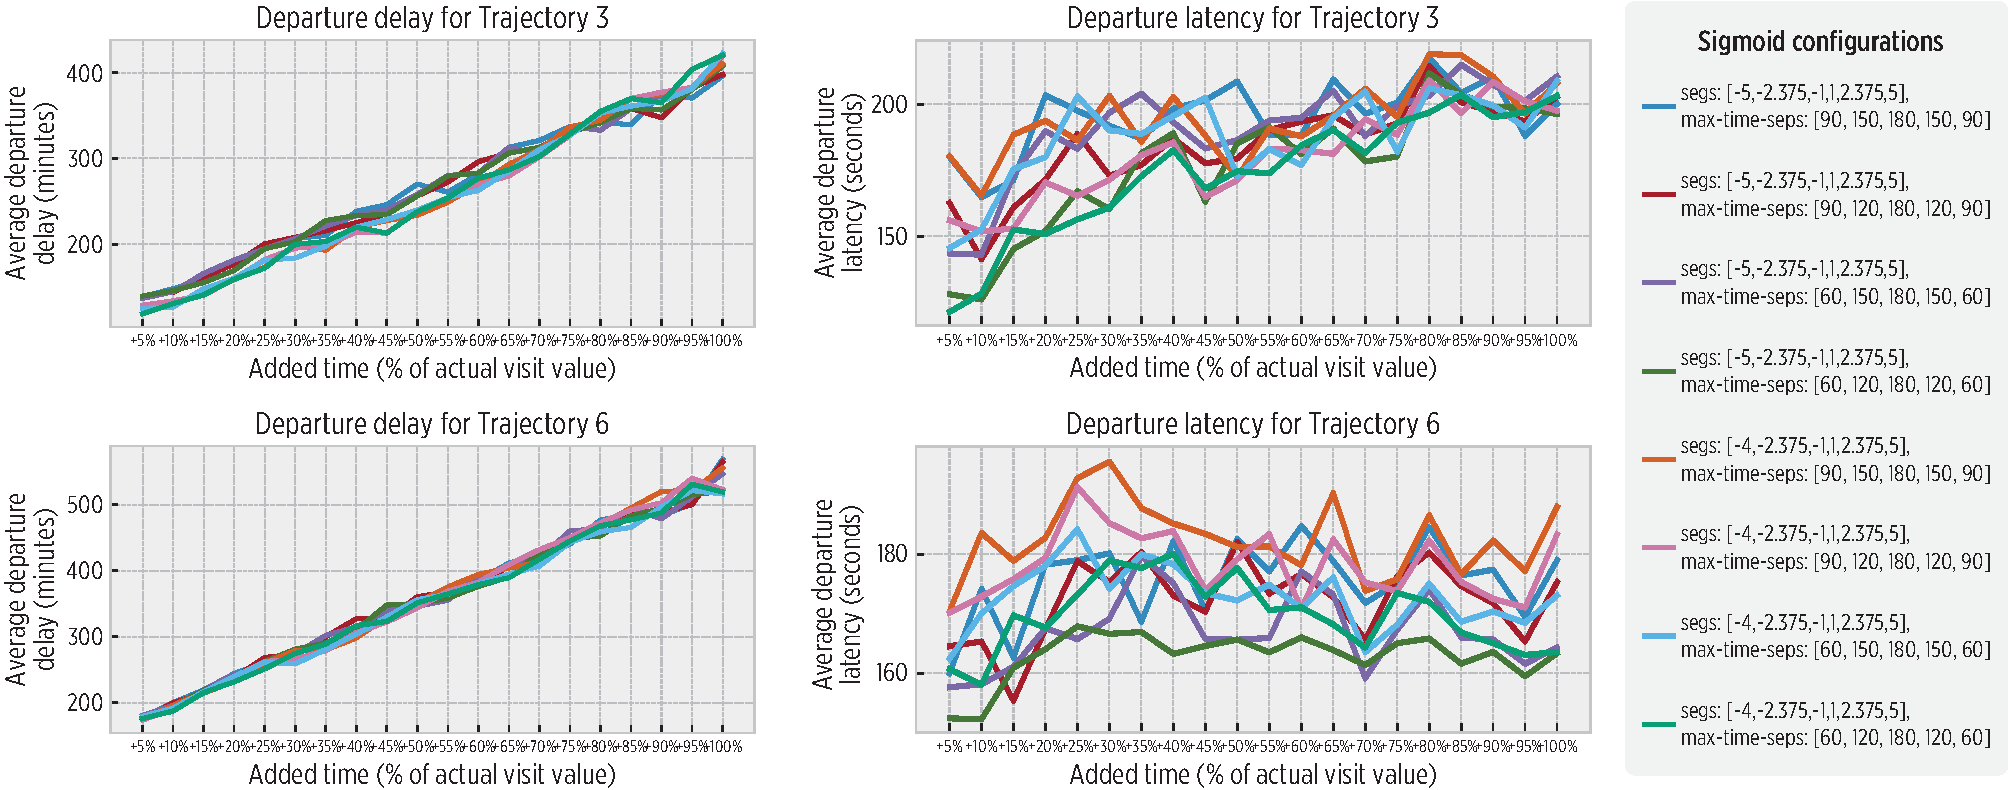
\includegraphics[width=1.05\textwidth]{vectors/experiments/exp-3/exp-3-b-departure-delay-and-latency}}%
  \caption{On the left, the evolution of the timespan between the expected and actual departures detected by the system when the STM is injured with additional time. Similar tendencies are observed, highlighting that the sigmoid sampling allows to identify that user is leaving the stay points before expected. 
  \\ On the right, the variation of the latency values of departures detection. The observed values are under the theoretical 360 seconds maximum peak}
\end{figure}
\end{frame}

% \begin{frame}{Preliminary experiments}{Reaction to STM mobility mismatches: Results}
% \begin{figure}
%   \centering
%   %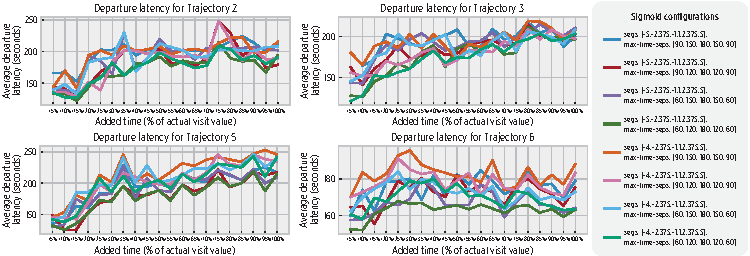
\includegraphics[width=\textwidth]{vectors/experiments/exp-3/exp-3-b-departure-latency-for-slides}
%   \makebox[\textwidth][c]{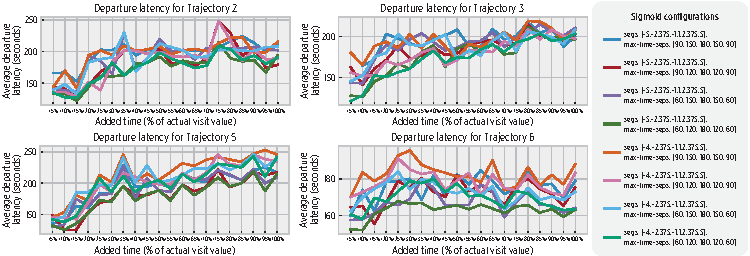
\includegraphics[width=1.05\textwidth]{vectors/experiments/exp-3/exp-3-b-departure-latency-for-slides}}%
%   \caption{The variation of the latency values of departures detection when the STM is injured with additional time. The observed values are under the theoretical 360 seconds maximum peak.}
%   \label{fig:exp-3-departure-latency}
% \end{figure}
% \end{frame}

% \subsection{Holistic evaluation}
\begin{frame}{Experimentation}{Holistic evaluation: Description}
\begin{block}{\small \textbf{Description}}
{ 
\small
\begin{itemize}
  \item This experiment was aimed at evaluating the overall spatial-time accuracy performance of the system with all of its component enabled, including:
  \begin{itemize}
    \item The continuous learning of stay points in the STM for adapting GPS sampling rate.
    \item The handling of mobility mismatches.
  \end{itemize}
\end{itemize}
}
\end{block}

\begin{table}
\centering
\renewcommand{\arraystretch}{0.8}
\resizebox{0.8\textwidth}{!}{%
\begin{tabular}{@{}lll@{}}
\toprule

\multirow{3}{*}{\textbf{Geofencing}} & \textbf{Radio distance} ($gf_{distance}$): & $250~m$ \\
 \cmidrule[0.25pt]{2-3}
 & \textbf{Window size} ($gf_{ws}$): & 3 \\

\cmidrule[0.25pt]{1-3}
\multirow{9}{*}{\textbf{Cognitive Controller}} & \multirow{2}{*}{\textbf{Sigmoid segments} ($\Theta_{domain\_segs}$):} & $(-5, -2.375), (-2.375, -1), (-1, 1), (1, 2.375), (2.375, 5)$ \\
 &  & $(-4, -2.375), (-2.375, -1), (-1, 1), (1, 2.375), (2.375, 5)$ \\
\cmidrule[0.25pt]{2-3}
 & \multirow{4}{*}{\textbf{Time separations} ($\Theta_{time\_sep}$):} & $[90, 150, 180, 150, 90]$ seconds \\
 &  & $[90, 120, 180, 120, 90]$ seconds \\
 &  & $[60, 150, 180, 150, 60]$ seconds \\
 &  & $[60, 120, 180, 120, 60]$ seconds \\
 \cmidrule[0.25pt]{2-3}
 & \textbf{On trajectory sampling}: & 30 seconds\\
 \cmidrule[0.25pt]{2-3}
 & \textbf{Conservative sampling}: & 60 seconds\\

\cmidrule[0.25pt]{1-3}
\textbf{Trajectories} & \multicolumn{2}{l}{All ground truth trajectories.} \\

\cmidrule[0.25pt]{1-3}
\textbf{STM} & \multicolumn{2}{l}{Empty}
\\
\bottomrule
\end{tabular}%
}
\caption{Input parameters for the holistic evaluation experiment. The \emph{conservative} sampling refers to the late departure mismatch reaction.}
\label{tab:exp-4-input-parameters}
\end{table}
\end{frame}


\begin{frame}{Experimentation}{Holistic evaluation: Results}
\small 
\vspace{-0.5cm}
{
  \centering
  \includegraphics[width=0.7\textwidth]{vectors/experiments/exp-4/exp-4-sigmoid-header-top-row}
  \par 
}

\begin{columns}
\begin{column}[T]{0.48\textwidth}
\begin{block}{\small \textbf{Arrival latency}}
{
  \centering
  \includegraphics[width=\textwidth]{vectors/experiments/exp-4/exp-4-arrival-latency-for-slides-v2}
  \captionof{figure}{Arrival latency observed by the platform in experimental trials. The largest average value is below 65 seconds, explained by the fact that 2 location updates must be collected by the \emph{Geofencing} module before identifying an arrival event.}
  \par 
}
\end{block}
\end{column}

\begin{column}[T]{0.52\textwidth}
\begin{block}{\small \textbf{Departure latency}}
{
  \centering
  \includegraphics[width=\textwidth]{vectors/experiments/exp-4/exp-4-departure-latency-for-slides-v2}
  \captionof{figure}{Departure latency observed by the platform across performed experimental trials. The latencies are within 65 and 165 seconds, which is aligned with the different values specified to the CC for its sigmoid-driven sampling.}
  \par
}
\end{block}
\end{column}
\end{columns}

\end{frame}



\begin{frame}{Experimentation}{Holistic evaluation: Results}
\small
\vspace{-0.5cm}
{
  \centering
  \includegraphics[width=0.7\textwidth]{vectors/experiments/exp-4/exp-4-sigmoid-header-top-row}
  \par 
}

\begin{columns}
\begin{column}[T]{0.5\textwidth}

\begin{block}{\small \textbf{Trajectory distance difference}}
{
  \centering
  \includegraphics[width=\textwidth]{vectors/experiments/exp-4/exp-4-on-trajectory-distance-for-slides-v2}
  \captionof{figure}{The average distance of equivalent trajectory segments during experimental trials. The values are enclosed within $2.5~m$ and $8.5~m$, with the 30 seconds sampling obtaining the lowest value in each trial.}
  \par
}
\end{block}

\end{column}

\begin{column}[T]{0.5\textwidth}
\begin{block}{\small \textbf{Overall reduction of location update requests}}
{
  \centering
  \includegraphics[width=\textwidth]{vectors/experiments/exp-4/exp-4-location-requests-for-slides-v2}
  \captionof{figure}{The proportion of location update requests employed by each experimental trial with respect to the corresponding $1~Hz$ ground truth trajectory. All of the parameter combinations outperform the 30 seconds sampling period, which provides a rough estimation of the energy savings that the system could achieve in on-device implementations.}
  \par
}
\end{block}
\end{column}
\end{columns}
\end{frame}

% \begin{frame}{Preliminary experiments}{Energy saving expectations of on-device stay points detection: Results}
% \small
% \begin{figure}
%   \centering
%   \includegraphics[width=\columnwidth]{vectors/local-poi-article/plot-energy-performance-r2-for-slides}
%   \caption{Energy performance comparison of on-device vs. MCC sample apps using different GPS sampling periods. Each of the on-device trials last longer than its corresponding remote implementation.}
%   \label{fig:energy-performance-on-device-mcc-comparison}
% \end{figure}
% \end{frame}

% \subsection{Energy consumption of fixed-sampling periods}
\begin{frame}{Experimentation}{Energy consumption of fixed-sampling periods: Description}
\small
\begin{block}{\small \textbf{Description}}
\begin{itemize}
  \item This experiment evaluated the impact of sampling adaptations based on fixed sampling rates on the energy consumed by the proposed CDS.
  \item All system components were enabled, with the exception of the sigmoid sampling of the CC.
  \item The CC followed fixed sampling periods depending on the current mobility state recognized by the system.
  \item The experiment also demonstrated the mobility awareness that the system provides to the smartphone (STM).
\end{itemize}
\end{block}


\begin{table}
\centering
\renewcommand{\arraystretch}{0.8}
\resizebox{0.7\textwidth}{!}{%
\begin{tabular}{@{}lll@{}}
\toprule
\multirow{2}{*}{\textbf{Stay Points Detector}} & \textbf{Time threshold} ($\delta_{time}$): & $45~min$ \\
\cmidrule[0.25pt]{2-3}
 & \textbf{Distance threshold} ($\delta_{distance}$): & $500~m$ \\

\cmidrule[0.25pt]{1-3}
\multirow{3}{*}{\textbf{Geofencing}} & \textbf{Radio distance} ($gf_{distance}$): & $250~m$ \\
% \cmidrule[0.25pt]{2-3}
% & \textbf{Pivot parameter} ($gf_{pv}$): & center \\
 \cmidrule[0.25pt]{2-3}
 & \textbf{Window size} ($gf_{ws}$): & 3 \\

\cmidrule[0.25pt]{1-3}
\multirow{2}{*}{\textbf{HAR module}} & \textbf{Individual window length}: & $5$ seconds \\
\cmidrule[0.25pt]{2-3}
 & \textbf{Meta-window size} ($HAR_{mws}$): & $5$ \\

\cmidrule[0.25pt]{1-3}
\multirow{4}{*}{\textbf{Cognitive Controller}} & \multirow{2}{*}{\textbf{Smartphone 1}:} & On trajectory sampling periods: 30 seconds\\
 &  & On stay point sampling period: 30 seconds \\
\cmidrule[0.25pt]{2-3}
 & \multirow{2}{*}{\textbf{Smartphone 2}:} & On trajectory sampling period: 30 seconds\\
 &  & \begin{tabular}[c]{@{}l@{}}On stay point sampling period:\\one in the set $\{ 60, 90, 120, 150, 180 \}$ seconds\end{tabular} \\

\bottomrule
\end{tabular}%
}
\caption{Input parameters for the energy consumption of fixed-sampling periods experiment.}
\end{table}
\end{frame}

\begin{frame}{Experimentation}{Energy consumption of fixed-sampling periods: Results}
\vspace{-0.4cm}
{
  \centering
  \includegraphics[width=0.85\textwidth]{vectors/experiments/exp-6/exp-6-energy-burnout}
  \captionof{figure}{Energy performance of a fixed 30 seconds sampling versus a basic sampling adaptation consisting in a 30 seconds sampling in trajectory mode and a slower sampling rate during stay point mode. The separation between the lines in each plot starts after the system learns the stay points with the largest weight in user mobility (home and work places).}
  \par
}
\end{frame}

\begin{frame}{Experimentation}{Energy consumption of fixed-sampling periods: Results}
\begin{figure}
  \includegraphics[width=0.8\textwidth]{vectors/experiments/exp-6/exp-6-map-trj-4-adaptive-sampling-60-sp}
  \caption{The information autonomously learned by the STM during the trial corresponding to the 30 seconds in trajectory and 60 seconds in stay point sampling scheme. The height of cylinders corresponds with the stay time during each stay point visit.}
  \label{fig:exp-6-stm-60-seconds-sp}
\end{figure}
\end{frame}


\begin{frame}{Experimentation}{Energy overhead of cognitive system}
\small
\vspace{-0.5cm}
\begin{columns}
\begin{column}[T]{0.55\textwidth}
\begin{block}{\small \textbf{Description}}
\begin{itemize}
  \item Evaluation of the energy overhead of the proposed CDS.
  \item A sample application was developed for collecting HAR + GPS data with a 30 seconds sampling rate.
  \item One smartphone unit instructed the sampling rate without using any cognitive feature.
  \item Another smartphone unit used the cognitive features with the exception of the cognitive controller.
\end{itemize}
\end{block}
\end{column}

\begin{column}[T]{0.45\textwidth}
\begin{table}
\centering
\renewcommand{\arraystretch}{0.8}
\resizebox{0.95\textwidth}{!}{%
\begin{tabular}{@{}lll@{}}
\toprule
\multirow{2}{*}{\textbf{Stay Points Detector}} & \textbf{Time threshold} ($\delta_{time}$): & $45~min$ \\
\cmidrule[0.25pt]{2-3}
 & \textbf{Distance threshold} ($\delta_{distance}$): & $500~m$ \\

\cmidrule[0.25pt]{1-3}
\multirow{3}{*}{\textbf{Geofencing}} & \textbf{Radio distance} ($gf_{distance}$): & $250~m$ \\
% \cmidrule[0.25pt]{2-3}
% & \textbf{Pivot parameter} ($gf_{pv}$): & center \\
 \cmidrule[0.25pt]{2-3}
 & \textbf{Window size} ($gf_{ws}$): & 3 \\

\cmidrule[0.25pt]{1-3}
\multirow{2}{*}{\textbf{HAR module}} & \textbf{Individual window length}: & $5$ seconds \\
\cmidrule[0.25pt]{2-3}
 & \textbf{Meta-window size} ($HAR_{mws}$): & $5$ \\

\cmidrule[0.25pt]{1-3}
\textbf{Cognitive Controller} & Disabled & \\
\bottomrule
\end{tabular}%
}
\caption{Input parameters for the energy overhead measurement experiment (\emph{Geofencing} and \emph{Stay Points Detector} enabled only in one smartphone).}
\end{table}
\end{column}
\end{columns}

\vspace{-0.3cm}
\begin{block}{\small \textbf{Results}}
{
  \centering
  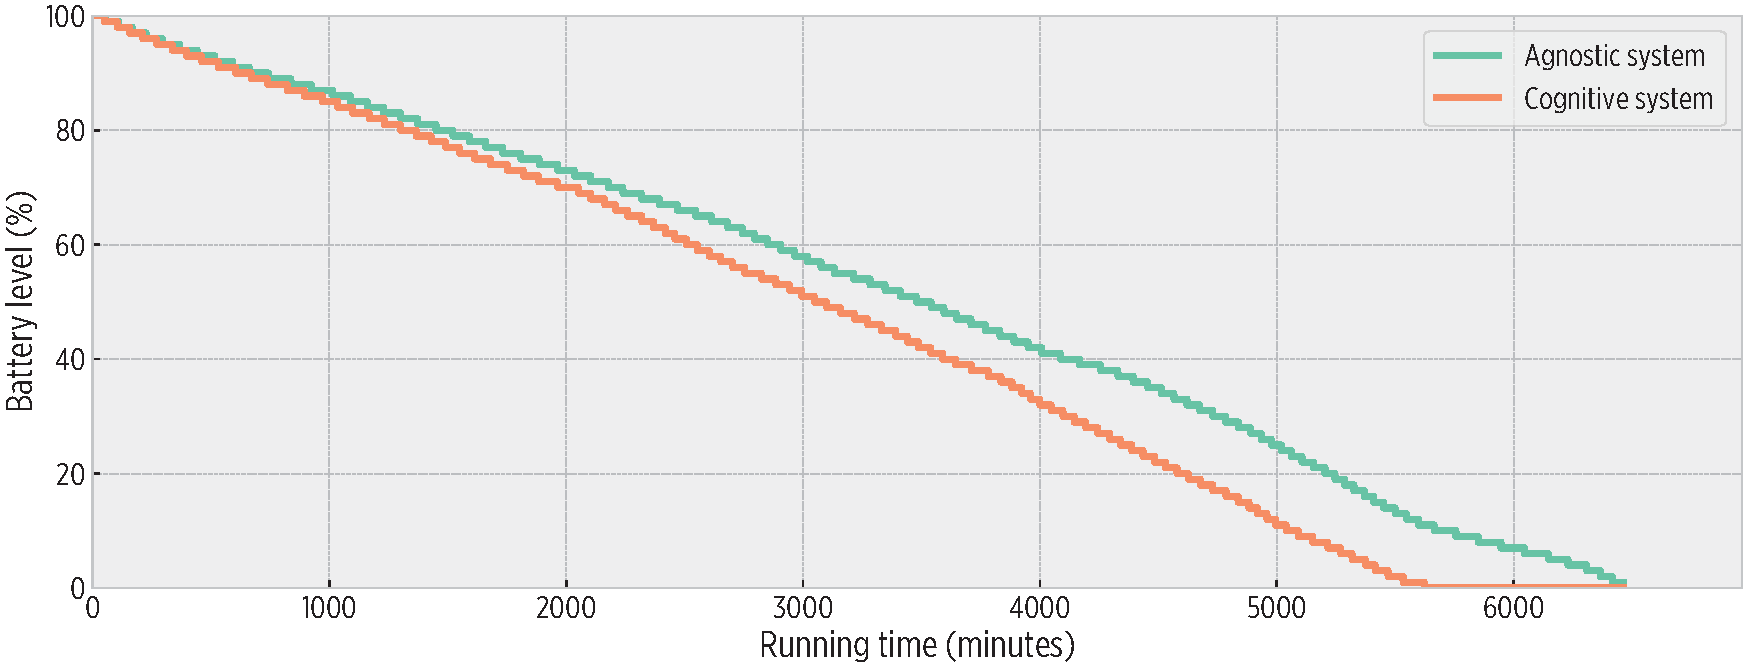
\includegraphics[width=0.7\textwidth]{vectors/experiments/energy-overhead}
  \captionof{figure}{Energy overhead of the cognitive system. The running time difference is about 14 hours.}
  \par
}
\end{block}

% \begin{table}
% \centering
% \renewcommand{\arraystretch}{0.8}
% \resizebox{0.45\textwidth}{!}{%
% \begin{tabular}{@{}lll@{}}
% \toprule
% \multirow{2}{*}{\textbf{Stay Points Detector}} & \textbf{Time threshold} ($\delta_{time}$): & $45~min$ \\
% \cmidrule[0.25pt]{2-3}
%  & \textbf{Distance threshold} ($\delta_{distance}$): & $500~m$ \\

% \cmidrule[0.25pt]{1-3}
% \multirow{3}{*}{\textbf{Geofencing}} & \textbf{Radio distance} ($gf_{distance}$): & $250~m$ \\
% % \cmidrule[0.25pt]{2-3}
% % & \textbf{Pivot parameter} ($gf_{pv}$): & center \\
%  \cmidrule[0.25pt]{2-3}
%  & \textbf{Window size} ($gf_{ws}$): & 3 \\

% \cmidrule[0.25pt]{1-3}
% \multirow{2}{*}{\textbf{HAR module}} & \textbf{Individual window length}: & $5$ seconds \\
% \cmidrule[0.25pt]{2-3}
%  & \textbf{Meta-window size} ($HAR_{mws}$): & $5$ \\

% \cmidrule[0.25pt]{1-3}
% \textbf{Cognitive Controller} & Disabled & \\
% \bottomrule
% \end{tabular}%
% }
% \caption{Input parameters for the energy overhead measurement experiment (Geofencing and Stay Points Detector enabled only in one smartphone).}
% \end{table}
\end{frame}

% \begin{frame}{Experimentation}{Energy overhead of cognitive system: Results}
% \small
% \begin{block}{Results}
% \begin{figure}
%   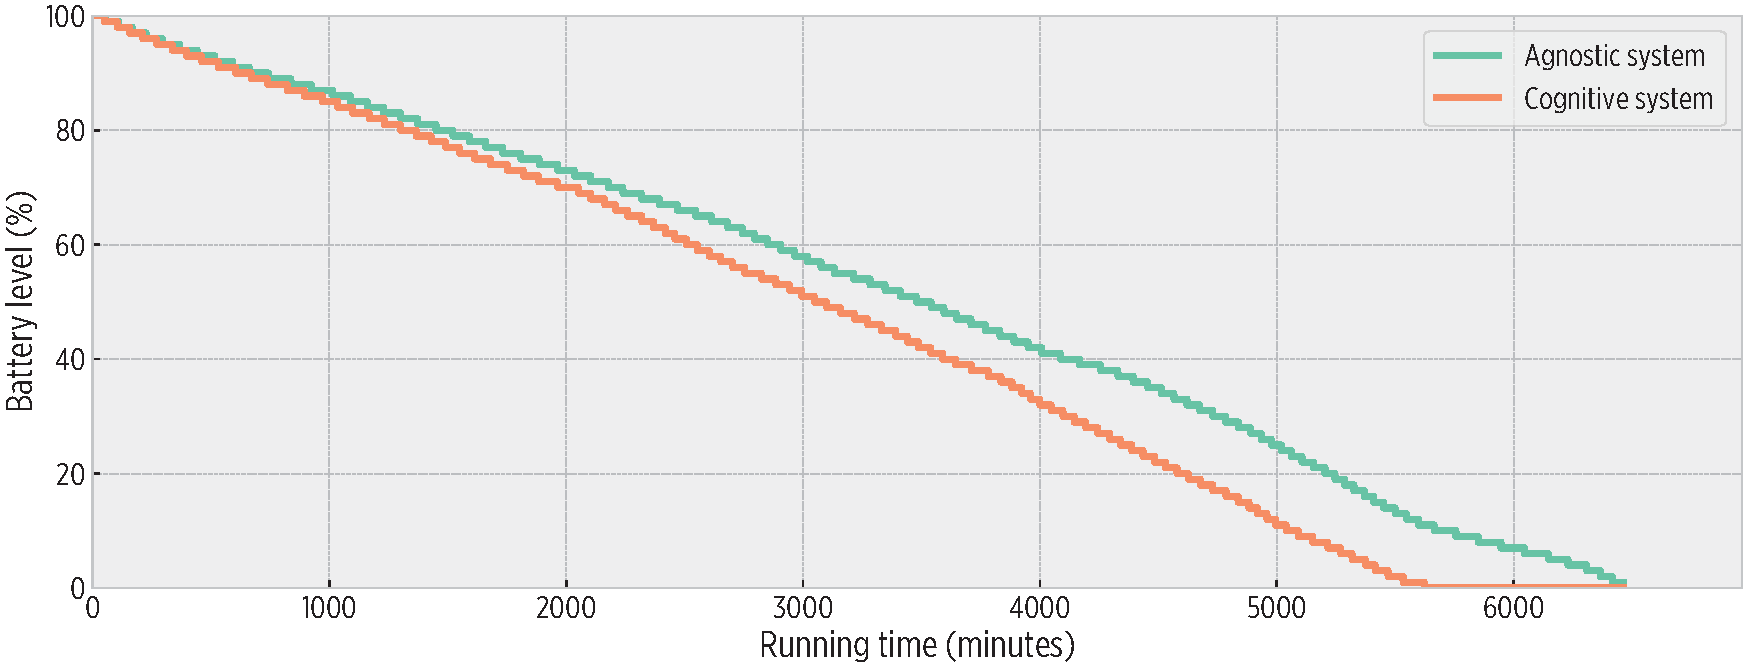
\includegraphics[width=\textwidth]{vectors/experiments/energy-overhead}
%   \caption{Energy overhead of the cognitive system. The running time difference is about 14 hours.}
% \end{figure}
% \end{block}
% \end{frame}

\section{Future work}
\label{sec:future_work}
The future work to be done in the next period is focused in the next activities.
%El trabajo futuro a realizar en el próximo periodo está enfocado en las siguientes actividades.

First, the verification and strength of the taxonomy of previous works presented in this report is going to be done.
%Primero, se realizará la verificación y enriquecimiento de la taxonomía de los trabajos del estado del arte presentada en este reporte.
This includes the revision of more and new articles reported in scientific magazines of the area, and the analysis of their technical and scientific details, in order to obtain a critical description of the approaches described inside them.
%Esto incluye la revisión de más y nuevos artículos reportados en revistas del área así como del análisis de los detalles técnicos y científicos con miras a preparar una descripción crítica de los métodos definidos en ellos.

Also, it is planned to analyze mobility data for defining and selecting the mobility patterns to be considered in this research work.
%Además, se planea el análisis de datos de movilidad para definir y seleccionar los patrones de movilidad a ser detectados en este trabajo de investigación.
The data are going to be captured through an Android mobile app which is also to be developed.
%Los datos serán capturados a través de una aplicación móvil Android que también está por desarrollarse.
This same data will be useful in the experimental stage of this research work.
%Estos mismos datos serán útiles para la etapa de experimentación en este trabajo de tesis.

Finally, it is planned to define the proper metrics for selecting the algorithms to perform the recognition of the mobility pattern from data described by the user.
%Finalmente, se definirán las métricas adecuadas para la selección de los algoritmos para realizar el reconocimiento de patrones, es decir los patrones de movilidad, a partir de los datos de movilidad descrita por el usuario.

Additionally, it is noteworthy that a subject related with data analysis and pattern recognition is going to be coursed, as suggested by the committee during the proposal research defense.
%Adicionalmente, es preciso mencionar que se cursará una materia relacionada con el análisis de datos y reconocimiento de patrones, tal como ha sido sugerido por el comité durante la defensa del protocolo de tesis.
This will be helpful to gain better scientific fundaments for concluding the state of art and perform the tasks previously described, that is the definition and selection of mobility patterns and the selection of the proper pattern recognition algorithms.
%Esto permitirá contar con mejores fundamentos científicos para la finalización del estado del arte y realizar las tareas descritas anteriormente, es decir la definición y selección de los patrones de movilidad y la selección de los algoritmos de reconocimiento de patrones.


{\aauwavesbg
\begin{frame}[plain,noframenumbering]
  \finalpage{
    Thank you for your attention!
  }
  { \tiny
    \epigraph{\tiny Consider again that dot [Earth]. That's here. That's home. That's us.}{\tiny \textit{Carl Sagan}}
  }
\end{frame}}

\begin{frame}[allowframebreaks,noframenumbering]
        \frametitle{References}
%\bibliographystyle{plain}
{
\tiny{}
\bibliographystyle{unsrt}
\bibliography{library}
}
\end{frame}

\begin{frame}{Research background}{Contributions}
\small
\begin{block}{\small \textbf{Contributions}}
\begin{itemize}
  \item An on-device mobility patterns detector that works with streams of raw data collected by smartphone's sensors (GPS and accelerometer).
  \item An on-device mobility analyzer that incrementally builds a model of user mobility from the detected mobility patterns.
  \item A cognitive controller inspired on CDSs that, based on the mobility information learned, dynamically adapts GPS sampling rate through power-aware policies. 
  \item A middleware with the previous modules embedded for easing the development of LBSs and MBSs for the Android mobile platform.
\end{itemize}
\end{block}
\end{frame}

{\aauwavesbg%
  \begin{textblock*}{5cm}(0.3cm,0.3cm)
  \small
  \textbf{The architecture of the proposed system implemented in the Android software stack.}
  \end{textblock*}
\begin{textblock*}{1cm}(12cm,9.3cm)
  \scriptsize
  \insertframenumber~/~\inserttotalframenumber
  \end{textblock*}
\begin{frame}[plain]
  \centering
  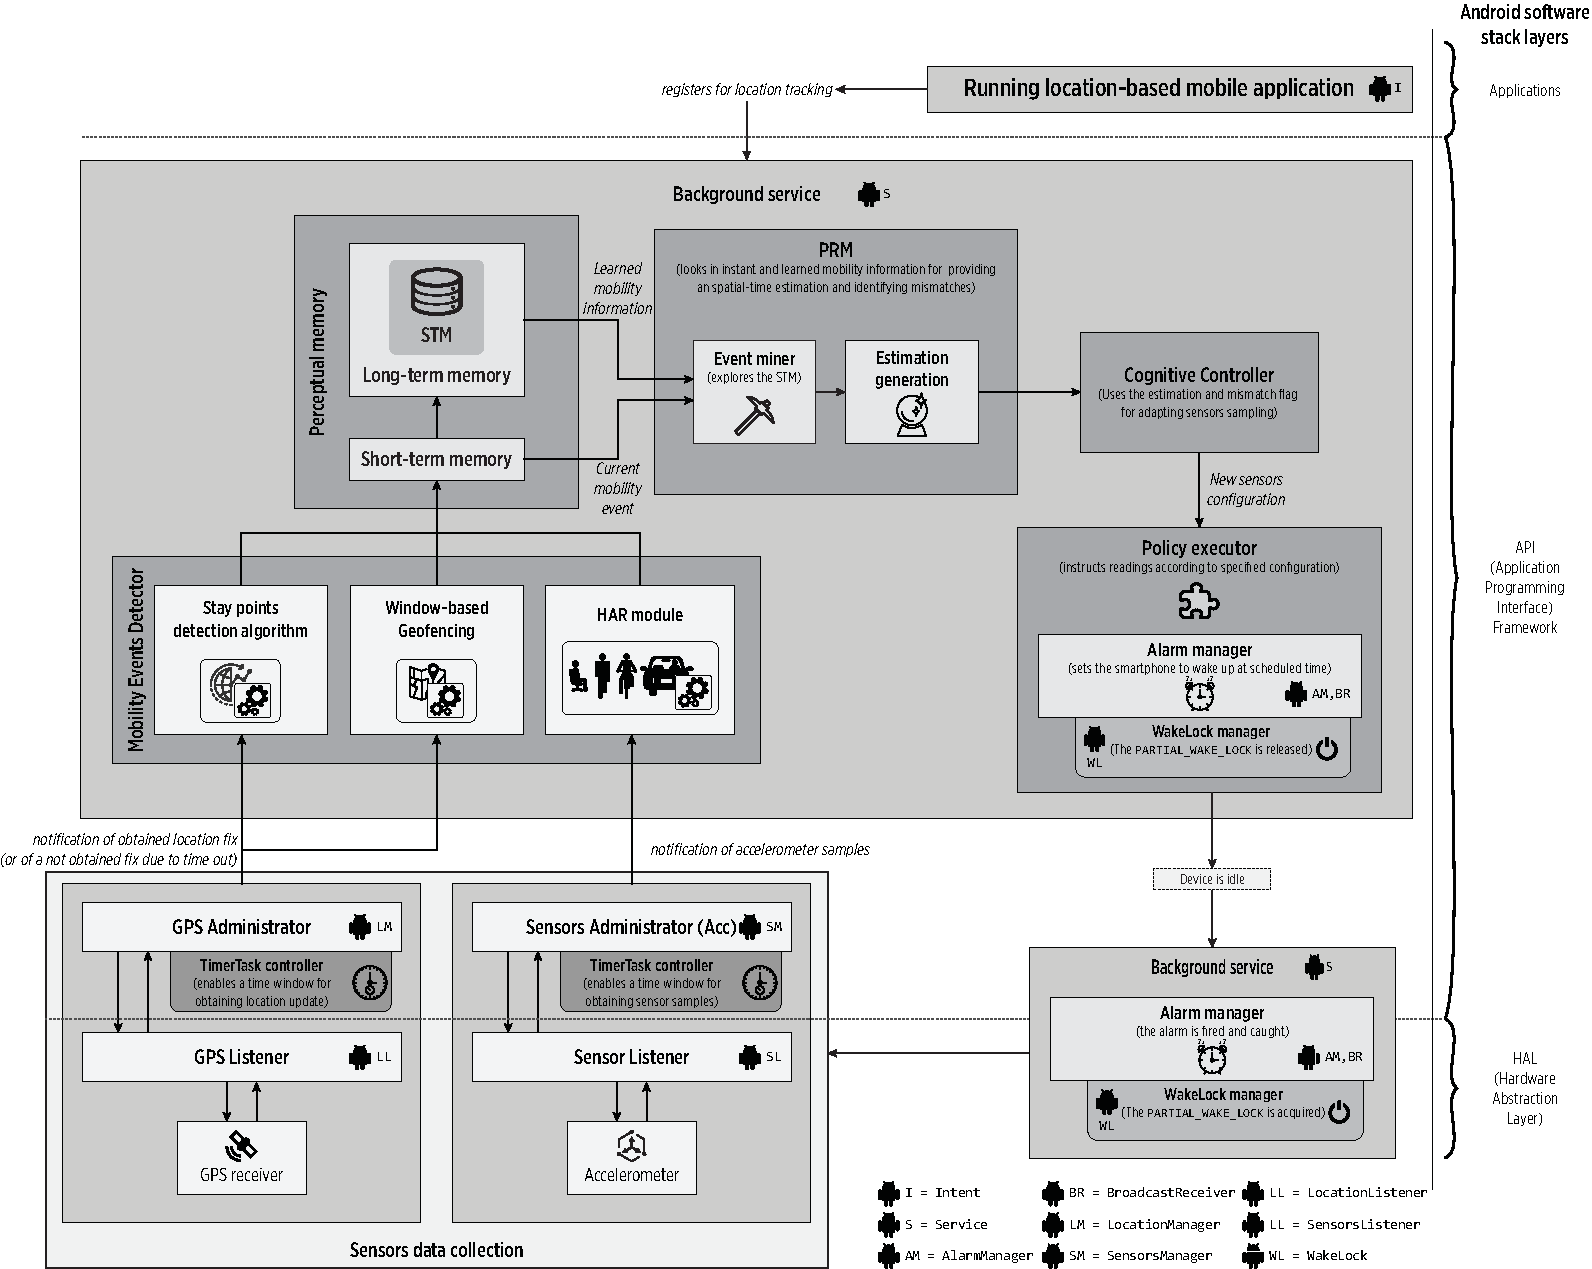
\includegraphics[width=\textwidth]{vectors/implementation}
\end{frame}}

\begin{frame}{Experimentation}{\emph{Stay Points Detector} module spatial-time accuracy: Results}
\vspace{-0.5cm}
\begin{table}
\centering
\renewcommand{\arraystretch}{0.8}
\resizebox{0.72\textwidth}{!}{%
\begin{tabular}{@{}lrrrrrr@{}}
\toprule
\multicolumn{1}{c}{\textbf{Trajectory}} & 
\multicolumn{1}{c}{\textbf{\begin{tabular}[c]{@{}c@{}}Sampling period\\(seconds)\end{tabular}}} & 
\multicolumn{1}{c}{\textbf{\begin{tabular}[c]{@{}c@{}}Live stay\\ points identified\end{tabular}}} & 
\multicolumn{1}{c}{\textbf{\begin{tabular}[c]{@{}c@{}}Average centroid\\ distance (meters)\end{tabular}}} & 
% \multicolumn{1}{c}{\textbf{\begin{tabular}[c]{@{}c@{}}Average diameter\\ distance (meters)\end{tabular}}} & 
% \multicolumn{1}{c}{\textbf{\begin{tabular}[c]{@{}c@{}}Average ST\\ difference (seconds)\end{tabular}}} & 
\multicolumn{1}{c}{\textbf{\begin{tabular}[c]{@{}c@{}}Average arrival\\ latency (seconds)\end{tabular}}} & 
\multicolumn{1}{c}{\textbf{\begin{tabular}[c]{@{}c@{}}Average departure\\ latency(seconds)\end{tabular}}} \\ 
\midrule
\multirow{6}{*}{Trajectory 1} 
 & 30 & 12 of 12 & 1.50 &   2.67 & 24.92 \\
 & 60 & 12 of 12 & 3.43 &   \textcolor{red}{\textbf{\emph{-12.33}}} & 17.42 \\
 & 90 & 12 of 12 & 4.04 &   15.17 & 32.42 \\
 & 120 & 12 of 12 & 6.66 &  \textcolor{red}{\textbf{\emph{-7.33}}} & 52.42 \\
 & 150 & 12 of 12 & 9.00 &  25.17 & 79.92 \\
 & 180 & 12 of 12 & 10.88 & 22.67 & 77.42 \\
 \cmidrule(l){1-6}

\multirow{6}{*}{Trajectory 2} 
 & 30 & 16 of 16 & 1.59 & 7.38 & 13.62 \\
 & 60 & 16 of 16 & 4.72 & 20.50 & 34.25 \\
 & 90 & 16 of 16 & 4.42 & 37.38 & 26.75 \\
 & 120 & 16 of 16 & 12.51 & 16.75 & 83.00 \\
 & 150 & 16 of 16 & 15.04 & \textcolor{red}{\textbf{\emph{-0.12}}} & 96.12 \\
 & 180 & 16 of 16 & 15.58 & 65.50 & 71.75 \\
 \cmidrule(l){1-6}

\multirow{6}{*}{Trajectory 3} 
 & 30 & 19 of 19 & 3.39 &  2.26 & 12.16 \\
 & 60 & 19 of 19 & 3.96 &  11.74 & 12.16 \\
 & 90 & 19 of 19 & 8.05 &  40.16 & 29.53 \\
 & 120 & 19 of 19 & 11.16  & 37.00 & 56.37 \\
 & 150 & 19 of 19 & 18.06  & 48.05 & 59.53 \\
 & 180 & 19 of 19 & \textcolor{green}{\textbf{22.52}} & 87.53 & 81.63 \\
 \cmidrule(l){1-6}

\multirow{6}{*}{Trajectory 4} 
 & 30 & 13 of 13 & 0.49 &  16.15 & 2.46 \\
 & 60 & 13 of 13 & 1.05 &  41.54 & 34.77 \\
 & 90 & 13 of 13 & 2.41 &  32.31 & 55.54 \\
 & 120 & 13 of 13 & 4.00 & 32.31 & 71.69 \\
 & 150 & 13 of 13 & 4.78 & 41.54 & 50.92 \\
 & 180 & 13 of 13 & 5.19 & 73.85 & 62.46 \\
 \cmidrule(l){1-6}

\multirow{6}{*}{Trajectory 5} 
 & 30 & 18 of 18 & 1.49 & 0.17 & 13.61 \\
 & 60 & 18 of 18 & 2.31 & 13.50 & 21.94 \\
 & 90 & 18 of 18 & 5.12 & \textcolor{red}{\textbf{\emph{-3.17}}} & 23.61 \\
 & 120 & 18 of 18 & 14.46 & 10.17 & \textcolor{red}{\textbf{\emph{-44.72}}} \\
 & 150 & 18 of 18 & 13.58 & 30.17 & \textcolor{red}{\textbf{\emph{-39.72}}} \\
 & 180 & 18 of 18 & 14.39 & 26.83 & \textcolor{red}{\textbf{\emph{-71.39}}} \\
 \cmidrule(l){1-6}

\multirow{6}{*}{Trajectory 6} 
 & 30 & 75 of 75 & 1.89 & 2.89 & 6.89 \\
 & 60 & \textcolor{blue}{\textbf{76 of 75}} & 3.54 & 8.49 & 24.89 \\
 & 90 & \textcolor{blue}{\textbf{76 of 75}} & 4.67  & 7.29 & 59.69 \\
 & 120 & \textcolor{blue}{\textbf{76 of 75}} & 6.71 & 29.29 & 77.69 \\
 & 150 & 75 of 75 & 9.33 & 42.89 & 113.29 \\
 & 180 & \textcolor{blue}{\textbf{76 of 75}} & 10.29 & 51.69 & 108.89 \\
 \bottomrule 
\end{tabular}
}
\caption{Spatial-time differences in detected stay points per sampling period (ST=stay time). The negative values in the ST difference and the arrival and departure latencies are caused by the combined effect of user mobility and sparse sampling rate on the \emph{StreamedZhen} algorithm, which generates stay points in subtly different coordinates with different time information.}
\end{table}
\end{frame}



\begin{frame}{Experimentation}{\emph{Geofencing} module spatial-time accuracy: Results}
\vspace{-0.5cm}
\begin{figure}
  \centering
  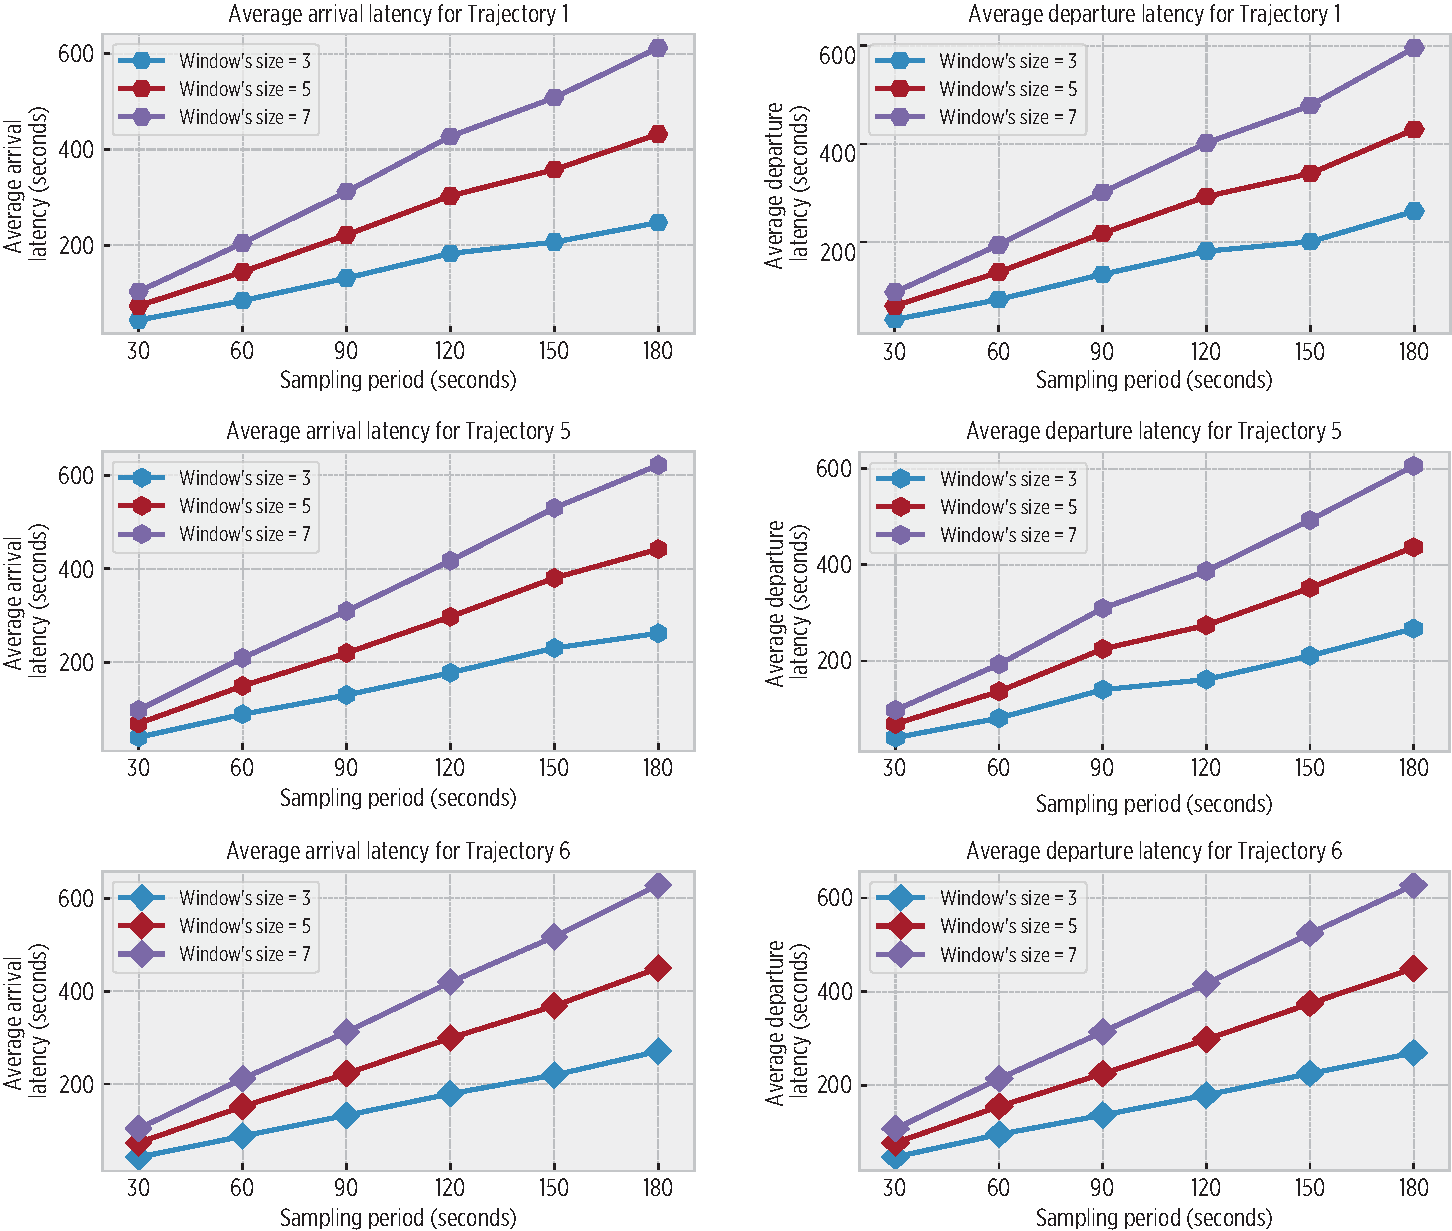
\includegraphics[width=0.75\textwidth]{vectors/experiments/exp-2/exp-2-latencies-for-slides}
  \caption{Arrival (left) and departure (right) latencies obtained by the Geofencing  module for each combination of sampling period and window length values. There is a tendency on the results as the shortest window’s sizes produce the shortest arrival latency values.}
\end{figure}
\end{frame}


\begin{frame}{Experimentation}{Holistic evaluation: Results}
\small 
\vspace{-0.5cm}
{
  \centering
  \includegraphics[width=0.7\textwidth]{vectors/experiments/exp-4/exp-4-sigmoid-header-top-row}
  \par 
}


\begin{columns}
\begin{column}[T]{0.5\textwidth}

\begin{block}{\small \textbf{Arrival distance difference}}
{
  \centering
  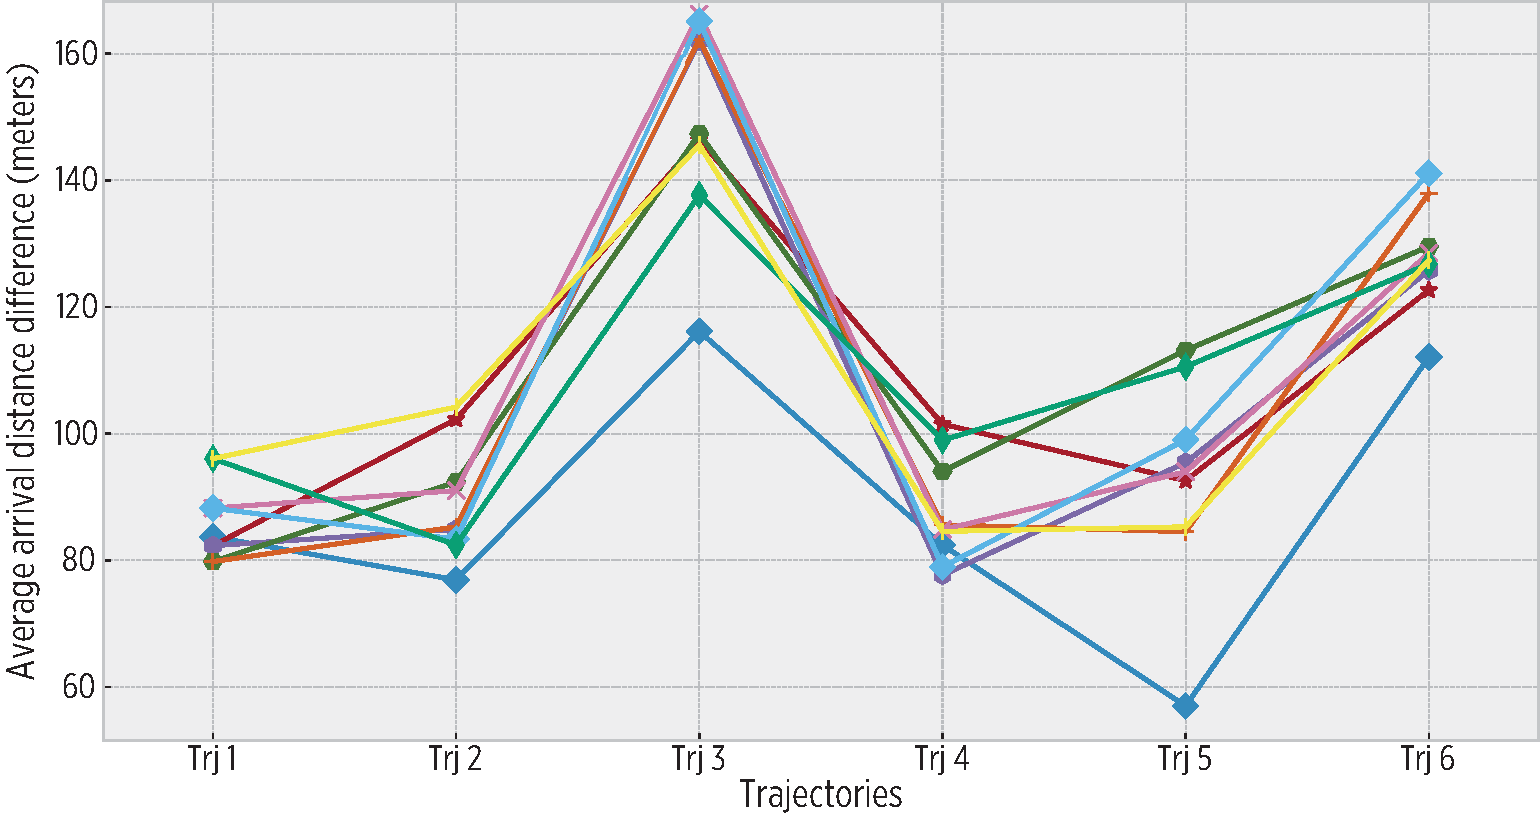
\includegraphics[width=\textwidth]{vectors/experiments/exp-4/exp-4-arrival-distance-for-slides-v2}
  \captionof{figure}{Arrival distance difference detected by the system throughout the different experimental trials. The values are shorter than for departure distance due to the decreasing speed that user describes when arriving to a stay point.}
  \par
}
\end{block}
\end{column}

\begin{column}[T]{0.5\textwidth}
\begin{block}{\small \textbf{Departure distance difference}}
{
  \centering
  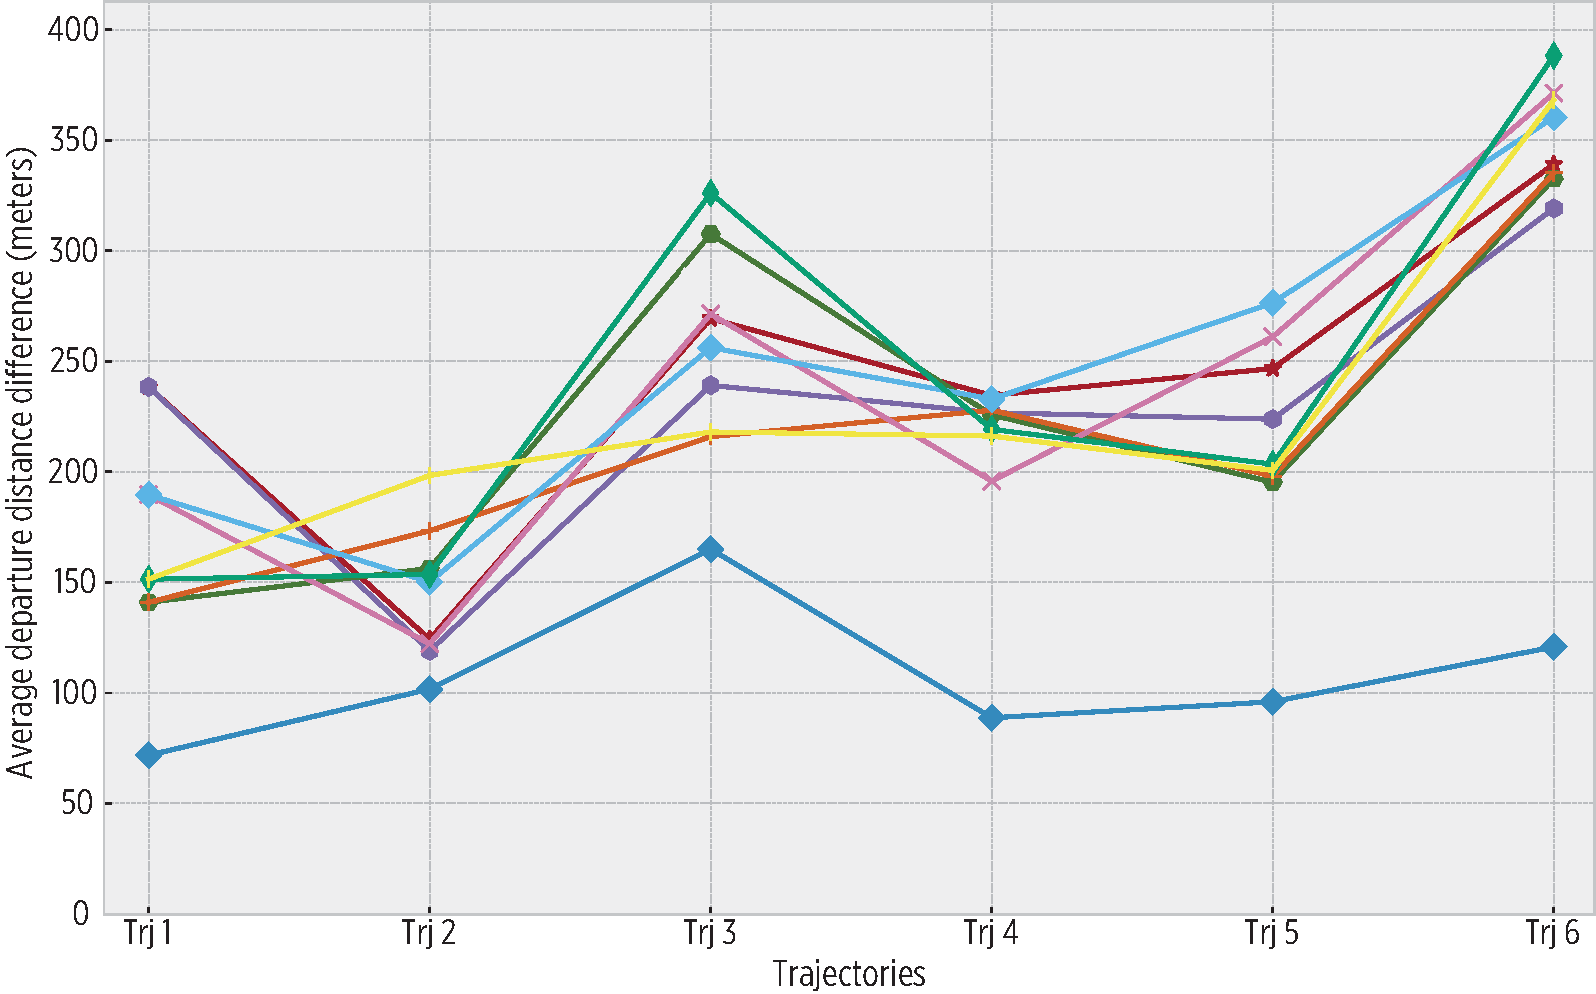
\includegraphics[width=\textwidth]{vectors/experiments/exp-4/exp-4-departure-distance-for-slides-v2}
  \captionof{figure}{Departure distance difference detected by the system throughout the different experimental trials. The larger distance differences are caused by the high speed with which user leaves the stay points (mostly using a vehicle as transportation mode).}
  \par
}
\end{block}

\end{column}
\end{columns}

\end{frame}


\begin{frame}{Experimentation}{Energy saving expectations of on-device stay points detection}
\small
% \vspace{-0.5cm}
\begin{columns}
\begin{column}{0.55\textwidth}
\begin{block}{\small \textbf{Description}}
\begin{itemize}
  \item This experiment explored whether a smartphone could detect stay points by itself, and the energy savings of such implementation with respect of typical Mobile Cloud Computing (MCC) based solutions.
  % \item Typical solutions implement a Mobile Cloud Computing (MCC) approach on which the smartphone only collects and offloads the processing to external servers.
\end{itemize}
\end{block}
\end{column}

\begin{column}{0.4\textwidth}
\begin{table}
\centering
\renewcommand{\arraystretch}{0.8}
\resizebox{0.95\textwidth}{!}{%
\begin{tabular}{lll}
\toprule
\multirow{2}{*}{\textbf{Stay Points Detector}} & \textbf{Time threshold} ($\delta_{time}$): & $45~min$ \\
\cmidrule[0.25pt]{2-3}
 & \textbf{Distance threshold} ($\delta_{distance}$): & $500~m$ \\

\cmidrule[0.25pt]{1-3}
\textbf{Sampling periods}: & \multicolumn{2}{l}{30, 60, 90, 120, 150 seconds} \\
\bottomrule
\end{tabular}
}
\caption{Input parameters for the energy saving expectations of on-device stay points detection experiment.}
\label{tab:exp-energy-performance-input-parameters}
\end{table}
\end{column}
\end{columns}

\begin{figure}
  \centering
  \includegraphics[width=\columnwidth]{vectors/local-poi-article/plot-energy-performance-r2-for-slides}
  \caption{Energy performance comparison of on-device vs. MCC sample apps using different GPS sampling periods. Each of the on-device trials last longer than its corresponding remote implementation.}
\end{figure}

\end{frame}


\begin{frame}{Experimentation}{Comparison with other solutions}
\begin{table}[]
\centering
\small
\renewcommand{\arraystretch}{1.2}
\begin{tabular}{@{}p{1cm}p{1.8cm}p{1.6cm}p{1.4cm}p{1cm}p{1cm}@{}}
\toprule
\textbf{Work} &
\textbf{Purpose} &
\textbf{Mobility type} &
\textbf{Involved sensors} &
\textbf{Trajectory tracking} &
\textbf{Place learning} \\ 
\midrule

\textbf{SenseLess} &
Location tracking &
Walking, static &
Accelerometer, GPS &
Yes &
No \\

\cmidrule[0.25pt]{1-6}
\textbf{SmartDC} &
Place tracking &
Not specified &
Cellular id, Wi-Fi, GPS&
No &
Yes \\

\cmidrule[0.25pt]{1-6}
Proposed system &
Location and place tracking &
Static, walking, biking, vehicle &
Accelerometer, GPS &
Yes &
Yes \\

\bottomrule
\end{tabular}%

\caption{Features comparison of proposed system and representative existing solutions.}
\end{table}
\end{frame}



% \begin{frame}[noframenumbering]{Detailed schedule}
% \begin{table}[]
% \centering
% \resizebox{0.95\textwidth}{!}{%
% \begin{tabular}{clccccccc}
%    &                                                                               & 2014 & \multicolumn{3}{c}{2015} & \multicolumn{3}{c}{2016}  \\
%    \cline{3-9}
% \multicolumn{2}{l}{\small{Work: \markdone~Done, \markonprogress~In progress, \markoff~To be done}} & 3rd & 1st & 2nd & 3rd & 1st & 2nd & 3rd \\
%    \toprule
% \multicolumn{2}{c}{\textsc{Step I}}                                                &  &  &  &  &  &  &  \\
% 1  & State-of-art reading                                                          & \markdone & \markdone &  &  &  &  &  \\
% 2  & State-of-art works categorization                                             &  & \markdone & \markdone  &  &  &  &  \\
% 3  & Documentation of information found (committee request)                        &  &  & \markdone &  &  &  &  \vspace{1em}\\

% \multicolumn{2}{c}{\textsc{Step II}}                                               &  &  &  &  &  &  &  \\
% 4  & \makecell[l]{Development of a mobile app for accelerometer and location \\data collection}    &  &  & \markdone & \markdone  &  &  &  \\
% 5  & Analysis of data                                                              &  &  &  & \markdone  &  &  &  \\
% 6  & Formal definition of mobility pattern                                         &  &  &  & \markdone &  &  &  \\
% 7  & Selection of mobility patterns                                                &  &  &  & \markdone & \markdone &  &  \vspace{1em}\\

% \multicolumn{2}{c}{\textsc{Step III}}                                              &  &  &  &  &  &  &  \\
% 8  & Research on classification algorithms for mobility patterns                   &  &  &  & \markdone & \markdone &  &  \\
% 9  & Definition of metrics for evaluating algorithms                               &  &  &  &  & \markdone &  &  \\
% 10 & Implementation of algorithms in mobile platform                               &  &  &  &  & \markdone & \markdone  &  \\
% 11 & Selection of best algorithms according to metrics                             &  &  &  &  &  & \markdone &  \vspace{1em}\\

% \multicolumn{2}{c}{\textsc{Step IV}}                                               &  &  &  &  &  &  &  \\
% 12 & Definition and modeling of parameters needed by the \emph{Mobility Events Detector}                       &  &  &  & \markdone & \markdone & \markdone & \markdone \\
% 13 & Development of the \emph{Mobility Events Detector}.  &  &  &  & \markdone & \markdone & \markdone & \markdone \\
% \bottomrule
% \end{tabular}%
% }
% \caption{Schedule of activities (each column represents a four months period)}
% \end{table}
% \end{frame}

% \begin{frame}[noframenumbering]{Detailed schedule}
% \begin{table}[]
% \centering
% \resizebox{0.95\textwidth}{!}{%
% \begin{tabular}{clccccccc}
%    &                                                                               & \multicolumn{3}{c}{2016} & \multicolumn{3}{c}{2017} & 2018 \\
%    \cline{3-9}
% \multicolumn{2}{l}{\small{Work: \markdone~Done, \markonprogress~In progress, \markoff~To be done}}   & 1st & 2nd & 3rd & 1st & 2nd & 3rd & 1st \\
%    \toprule
% \multicolumn{2}{c}{\textsc{Step V}}                                                &  &  &  &  &  &  & \\
% 14  & Formal definition of policy                                                  &  &  & \markdone &  &  &  & \\
% 15  & \makecell[l]{Research and evaluation of techniques for\\generation and adaption of policies}&  &  & \markdone & \markdone  &  &  & \\
% 16  & Design and execution of experiments applied to use cases                     &  &  & \markdone & \markdone  &  &  & \\
% 17  & Selection of policies                                                        &  &  &  & \markdone  &  &  & \vspace{1em} \\

% \multicolumn{2}{c}{\textsc{Step VI}}                                               &  &  &  &  &  &  & \\
% 18  & Definition and modeling of Cognitive Controller parameters                                    &  &  &  &  & \markdone  &  & \\
% 19  & Development of the Cognitive controller                                                          &  &  &  &  & \markdone  &  & \vspace{1em} \\

% \multicolumn{2}{c}{\textsc{Step VII}}                                               &  &  &  &  &  &  & \\
% 20  & Analysis of components into software abstractions                             &  &  &  &  & \markdone  &  & \\
% 21  & Research on Android API for specialized components                            &  &  &  &  & \markdone  &  & \\
% 22  & Development of middleware                                                     &  &  &  &  & \markdone  &  & \vspace{1em}\\

% \multicolumn{2}{c}{\textsc{Step VIII}}                                              &  &  &  &  &  &  & \\
% 23  & \makecell[l]{Definition of experiments aimed at accuracy\\and energy consumption metrics}    &  &  &  &  &  & \markdone & \\
% 24  & Development of experimental sample mobile apps                                &  &  &  &  &  & \markonprogress & \\
% 25  & Experiments execution                                                         &  &  &  &  &  & \markonprogress & \markoff  \\
% 26  & Final results analysis                                                              &  &  &  &  &  &  & \markoff \\
% \bottomrule
% \end{tabular}%
% }
% \caption{Schedule of activities (each column represents a four months period)}
% \end{table}
% \end{frame}

% \begin{frame}[noframenumbering]{Detailed schedule}
% \begin{table}
% \centering
% \resizebox{\textwidth}{!}{%
% \begin{tabular}{clcccccccccccc}
%    &                                                                               & 2014 & \multicolumn{3}{c}{2015} & \multicolumn{3}{c}{2016} & \multicolumn{3}{c}{2017} & \multicolumn{2}{c}{2018} \\
%    \cline{3-14}
%  \multicolumn{2}{l}{\small{Work: \markdone~Done, \markonprogress~In progress, \markoff~To be done}} & 3rd & 1st & 2nd & 3rd & 1st & 2nd & 3rd & 1st & 2nd & 3rd & 1st & 2nd\\
%    \toprule
% \multicolumn{2}{c}{\textsc{Required tasks}}                                        &  &  &  &  &  &  &  &  &  &  &  & \\
% A   & Related courses                                                              & \markdone  & \markdone  & \markdone &  &  &  &  &  &  &  &  & \\
% B   & Research articles submission                                                 &  &  &  & \markdone &  & \markdone &  &  &  &  & \markonprogress & \\
% C   & Predoctoral exam preparation                                                 &  &  &  &  &  &  &  &  & \markdone &  &  & \\
% D   & Thesis writing                                                               & \markdone  &  &  & \markdone &  &  & \markdone &  &  & \markonprogress & \markoff & \markoff \\

% \bottomrule
% \end{tabular}%
% }
% \caption{Schedule of required activities}
% \end{table}
% \end{frame}


% \begin{frame}[noframenumbering]{Layered perceptual memory}{Short and long-term memory information}
% \vspace{-0.25cm}
% \small
% \begin{block}{\small \textbf{Layered perceptual memory}}
% \begin{itemize}
%     \item Short-term memory information: current (observed) mobility status.
%     \item Long-term memory information: the Expanded Spatial-Time model (STM).
% \end{itemize}
% \end{block}

% \begin{block}{\small \textbf{Expanded Spatial-Time model}}
% \begin{itemize}
%   \item The highest level of mobility information held by the system.
% \end{itemize}
% {
%   \centering
%   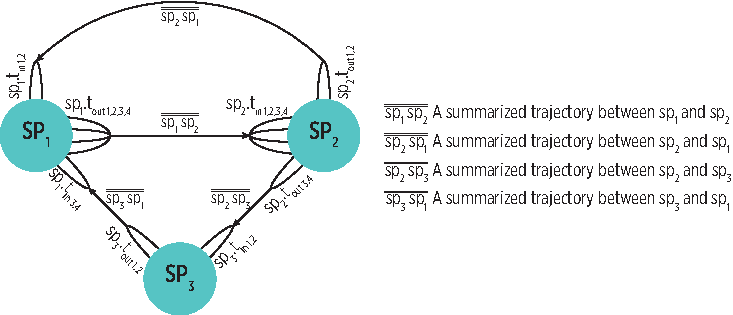
\includegraphics[width=0.75\textwidth]{vectors/stm-slides}
%   \captionof{figure}{A conceptual representation of the STM's structure.}
% \par }
% \end{block}
% \end{frame}

% \begin{frame}[noframenumbering]{Layered perceptual memory}{Expanded Spatial-Time model (STM)}
% \small
% \begin{block}{\small \textbf{Generation of the STM}}
% \begin{itemize}
%     \item Incrementally built with the coarse-grain mobility events detected by the \emph{Mobility Events Detector}.
% \end{itemize}
% {
%   \centering
%   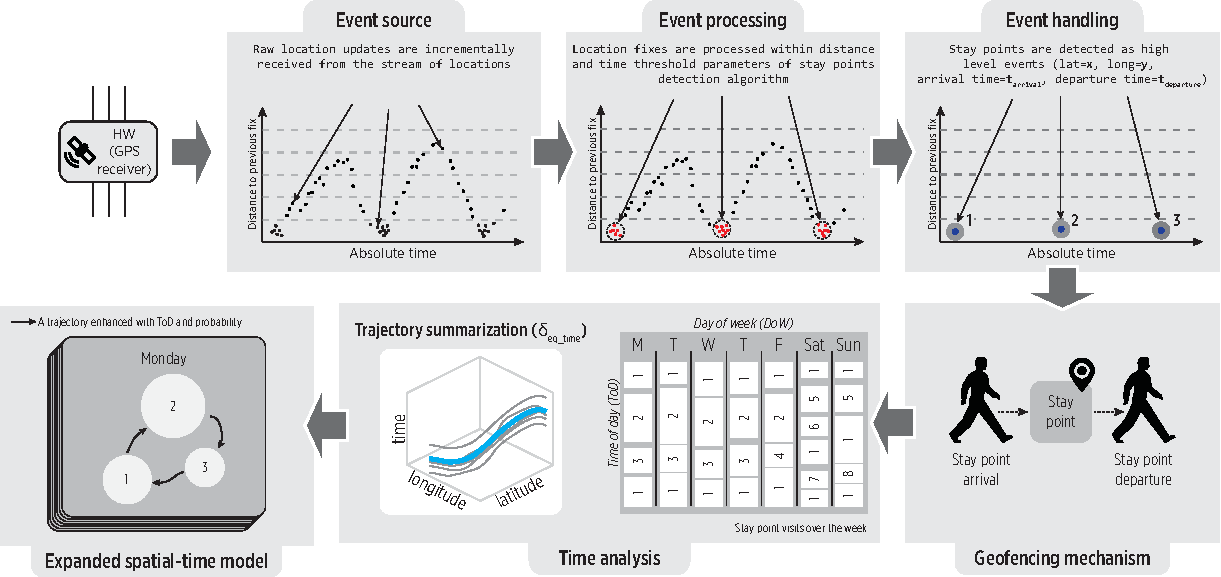
\includegraphics[width=\textwidth]{vectors/event-driven-memory-generation-for-slides}
%   \captionof{figure}{A conceptual representation of the steps for generating the STM from raw sensors data.}
%   \par
% }
% \end{block}
% \end{frame}


% \begin{frame}[noframenumbering]{Cognitive controller (CC)}{Description}
% \small
% \vspace{-0.5cm}
% \begin{columns}
% \begin{column}[T]{0.5\textwidth}
% \begin{block}{\small \textbf{Goals}}
%   \begin{itemize}
%       \item To reduce the energy consumption of location tracking by relying on PRM's estimations.
%       \item To reduce the system uncertainty about current user mobility.
%   \end{itemize}
% \end{block}
% \end{column}

% \begin{column}[T]{0.5\textwidth}
% \begin{block}{\small \textbf{Possible cognitive actions}}
%   \begin{itemize}
%     \item \textbf{Exploitation policies}: When system uncertainty is low for saving energy purposes.
%     \item \textbf{Exploration policies}: When system uncertainty is high for recovering for accuracy loss.
%   \end{itemize}
% \end{block}
% \end{column}
% \end{columns}

% \begin{figure}
%   \centering
%   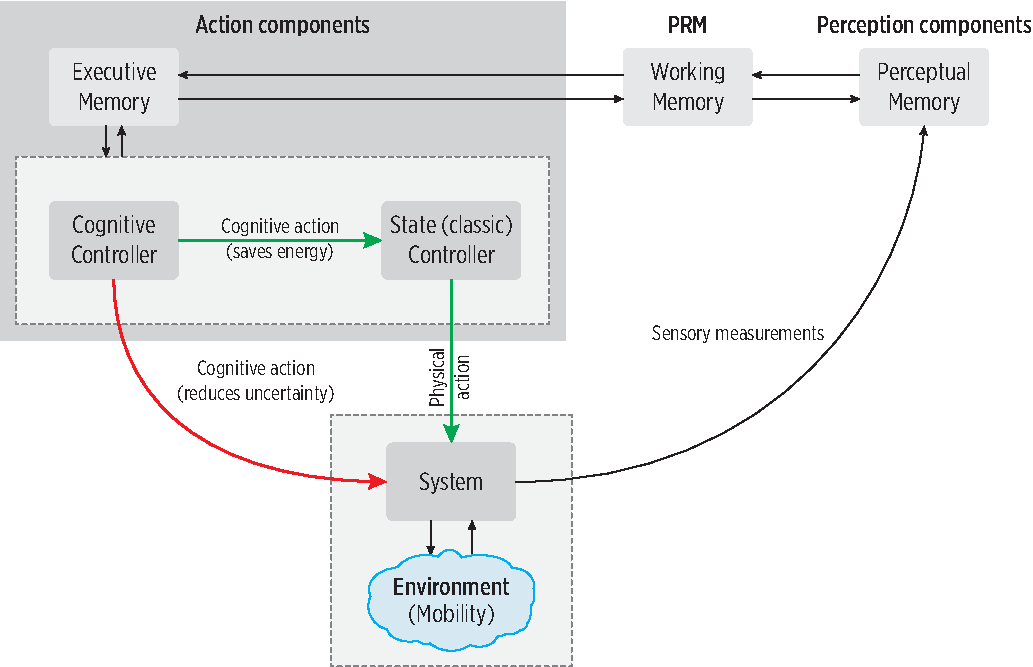
\includegraphics[width=0.65\textwidth]{vectors/cognitive-controller-architecture}
%   \caption{A generic cognitive controller architecture}
% \end{figure}
% \end{frame}

% \begin{frame}[noframenumbering]{Cognitive controller}{Policies tailored for user mobility}
% \small
% \begin{block}{\small \textbf{Stay point mode}}
%   \begin{itemize}
%       \item A sampling based on the sigmoid function $sig(x) = \frac{1}{1+e^{-\alpha x}}$ as a model for the mobility phase transitions.
%       \item Higher sampling rate on arrival and departure, when the user is more likely to move, and slower at the middle of a visit.
%   \end{itemize}
% \end{block}

% \begin{columns}
% \begin{column}{0.45\textwidth}
% \begin{figure}
%   \centering
%   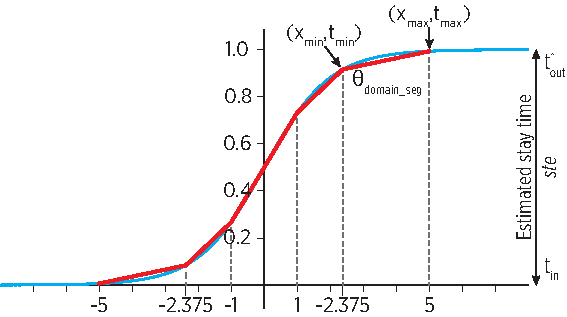
\includegraphics[width=0.99\linewidth]{vectors/sigmoid-segmentation-for-slides}
%   \caption{Approximation of the sigmoid through straight segments.}
% \end{figure}
% \end{column}

% \begin{column}{0.55\textwidth}
% \begin{figure}
%   \centering
%   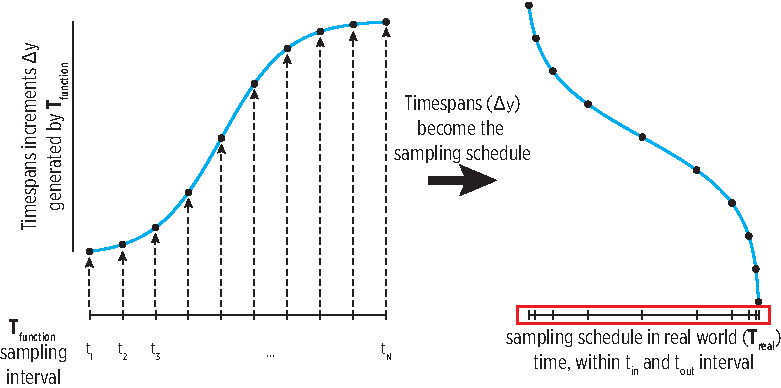
\includegraphics[width=0.99\linewidth]{vectors/sigmoid-driven-sampling-policy-for-slides}
%   \caption{A snapshot of the process for producing a sigmoid sampling.}
% \end{figure}
% \end{column}
% \end{columns}
% \end{frame}

% \begin{frame}[noframenumbering]{Preliminary experimentation}{\emph{Stay Points Detector} module spatial-time accuracy}
% \small

% \begin{columns}
% \begin{column}[T]{0.55\textwidth}

% \begin{block}{\small \textbf{Description}}
% \begin{itemize}
%   \item This experiment evaluates the spatial-time accuracy of the \emph{Stay Points Detector} module under different GPS sampling rates in terms of centroid distances and latencies.
% \end{itemize}
% \end{block}

% \end{column}
% \begin{column}[T]{0.45\textwidth}
% \begin{table}
% \centering
% \renewcommand{\arraystretch}{0.6}
% \resizebox{0.9\textwidth}{!}{%
% \begin{tabular}{lll}
% \toprule
% \multirow{2}{*}{\textbf{Stay Points Detector}} & \textbf{Time threshold} ($\delta_{time}$): & $45~min$ \\
% \cmidrule[0.25pt]{2-3}
%  & \textbf{Distance threshold} ($\delta_{distance}$): & $500~m$ \\

% \cmidrule[0.25pt]{1-3}
% \textbf{Sampling periods}: & \multicolumn{2}{l}{30, 60, 90, 120, 150, 180 seconds.} \\

% \cmidrule[0.25pt]{1-3}
% \textbf{Trajectories}: & \multicolumn{2}{l}{All ground truth trajectories.} \\
% \bottomrule
% \end{tabular}
% }
% \caption{Input parameters for the spatial-time accuracy of stay points experiment.}
% \end{table}
% \end{column}
% \end{columns}

% \vspace{-0.5cm}
% \begin{block}{\small \textbf{Results}}
% \begin{columns}
% \begin{column}{0.65\textwidth}
% \begin{figure}
%   \centering
%   \includegraphics[width=0.99\textwidth]{vectors/exp-1-centroid-distance}
% \end{figure}
% \end{column}
% \begin{column}{0.3\textwidth}
% \captionof{figure}{The impact of different sampling periods on the centroid distance of identified stay points in each trajectory. A maximum centroid distance of $22.52~m$ is identified when employing the 180 seconds sampling period.}
% \end{column}
% \end{columns}

% \end{block}
% \end{frame}


% \begin{frame}[noframenumbering]{Preliminary experimentation}{\emph{Geofencing} module spatial-time accuracy: Results}
% \vspace{-0.5cm}
% \begin{figure}
%   \centering
%   \includegraphics[width=0.78\textwidth]{vectors/exp-2-visits-for-slides}
%   \caption{Visits missed by the \emph{Geofencing} module for each combination of sampling period and window size values. The largest amount is obtained for the \emph{Trajectory 6}, given its length (more than 30 days). Nevertheless, they do not account for a considerable time in overall trajectories.}
% \end{figure}
% \end{frame}


% \begin{frame}[noframenumbering]{Preliminary experimentation}{Holistic evaluation: Results}
% \small 
% \vspace{-0.5cm}
% {
%   \centering
%   \includegraphics[width=0.7\textwidth]{vectors/exp-4-sigmoid-header-top-row}
%   \par 
% }

% \begin{columns}
% \begin{column}[T]{0.48\textwidth}
% \begin{block}{\small \textbf{Arrival latency}}
% {
%   \centering
%   \includegraphics[width=\textwidth]{vectors/exp-4-arrival-latency-for-slides-v2}
%   \captionof{figure}{Arrival latency observed by the platform in experimental trials. The largest average value is below 65 seconds, explained by the fact that 2 location updates must be collected by the \emph{Geofencing} module before identifying an arrival event.}
%   \par 
% }
% \end{block}
% \end{column}

% \begin{column}[T]{0.52\textwidth}
% \begin{block}{\small \textbf{Departure latency}}
% {
%   \centering
%   \includegraphics[width=\textwidth]{vectors/exp-4-departure-latency-for-slides-v2}
%   \captionof{figure}{Departure latency observed by the platform across performed experimental trials. The latencies are within 65 and 165 seconds, which is aligned with the different values specified to the CC for its sigmoid-driven sampling.}
%   \par
% }
% \end{block}
% \end{column}
% \end{columns}
% \end{frame}

% \begin{frame}[noframenumbering]{Preliminary experimentation}{Holistic evaluation: Results}
% \small
% \vspace{-0.5cm}
% {
%   \centering
%   \includegraphics[width=0.7\textwidth]{vectors/exp-4-sigmoid-header-top-row}
%   \par 
% }

% \begin{columns}
% \begin{column}[T]{0.5\textwidth}

% \begin{block}{\small \textbf{Trajectory distance difference}}
% {
%   \centering
%   \includegraphics[width=\textwidth]{vectors/exp-4-on-trajectory-distance-for-slides-v2}
%   \captionof{figure}{The average distance of equivalent trajectory segments during experimental trials. The values are enclosed within $2.5~m$ and $8.5~m$, with the 30 seconds sampling obtaining the lowest values in each trial.}
%   \par
% }
% \end{block}

% \end{column}

% \begin{column}[T]{0.5\textwidth}
% \begin{block}{\small \textbf{Overall reduction of location update requests}}
% {
%   \centering
%   \includegraphics[width=\textwidth]{vectors/exp-4-location-requests-for-slides-v2}
%   \captionof{figure}{The proportion of location update requests employed by each experimental trial with respect to the corresponding $1~Hz$ ground truth trajectory. All of the parameter combinations outperform the 30 seconds sampling period, which provides a rough estimation of the energy savings that the system could achieve in on-device implementations.}
%   \par
% }
% \end{block}
% \end{column}
% \end{columns}
% \end{frame}

% \begin{frame}[noframenumbering]{Preliminary experimentation}{Energy saving expectations of on-device stay points detection}
% \small
% % \vspace{-0.5cm}
% \begin{columns}
% \begin{column}{0.55\textwidth}
% \begin{block}{\small \textbf{Description}}
% \begin{itemize}
%   \item This experiment explored whether a smartphone could detect stay points by itself, and the energy savings of such implementation with respect of typical Mobile Cloud Computing (MCC) based solutions.
%   % \item Typical solutions implement a Mobile Cloud Computing (MCC) approach on which the smartphone only collects and offloads the processing to external servers.
% \end{itemize}
% \end{block}
% \end{column}

% \begin{column}{0.4\textwidth}
% \begin{table}
% \centering
% \renewcommand{\arraystretch}{0.8}
% \resizebox{0.95\textwidth}{!}{%
% \begin{tabular}{lll}
% \toprule
% \multirow{2}{*}{\textbf{Stay Points Detector}} & \textbf{Time threshold} ($\delta_{time}$): & $45~min$ \\
% \cmidrule[0.25pt]{2-3}
%  & \textbf{Distance threshold} ($\delta_{distance}$): & $500~m$ \\

% \cmidrule[0.25pt]{1-3}
% \textbf{Sampling periods}: & \multicolumn{2}{l}{30, 60, 90, 120, 150 seconds} \\
% \bottomrule
% \end{tabular}
% }
% \caption{Input parameters for the energy saving expectations of on-device stay points detection experiment.}
% \end{table}
% \end{column}
% \end{columns}

% \begin{figure}
%   \centering
%   \includegraphics[width=\columnwidth]{vectors/plot-energy-performance-r2-for-slides}
%   \caption{Energy performance comparison of on-device vs. MCC sample apps using different GPS sampling periods. Each of the on-device trials last longer than its corresponding remote implementation.}
% \end{figure}

% \end{frame}


% \begin{frame}[noframenumbering]{Preliminary experimentation}{Energy consumption of fixed-sampling periods: Results}
% \vspace{-0.4cm}
% {
%   \centering
%   \includegraphics[width=0.85\textwidth]{vectors/exp-6-energy-burnout}
%   \captionof{figure}{Energy performance of a fixed 30 seconds sampling versus a basic sampling adaptation consisting in a 30 seconds sampling in trajectory mode and a slower sampling rate during stay point mode. The separation between the lines in each plot starts after the system learns the stay points with the largest weight in user mobility (home and work places).}
%   \par
% }
% \end{frame}


% \begin{frame}[noframenumbering]{Preliminary experimentation}{Energy consumption of fixed-sampling periods: Results}
% \vspace{-0.4cm}
% {
%   \centering
%   %\includegraphics[width=0.85\textwidth]{vectors/exp-6-energy-burnout}
%   %\captionof{figure}{Energy performance of a fixed 30 seconds sampling versus a basic sampling adaptation consisting in a 30 seconds sampling in trajectory mode and a slower sampling rate during stay point mode. The separation between the lines in each plot starts after the system learns the stay points with the largest weight in user mobility (home and work places).}
%   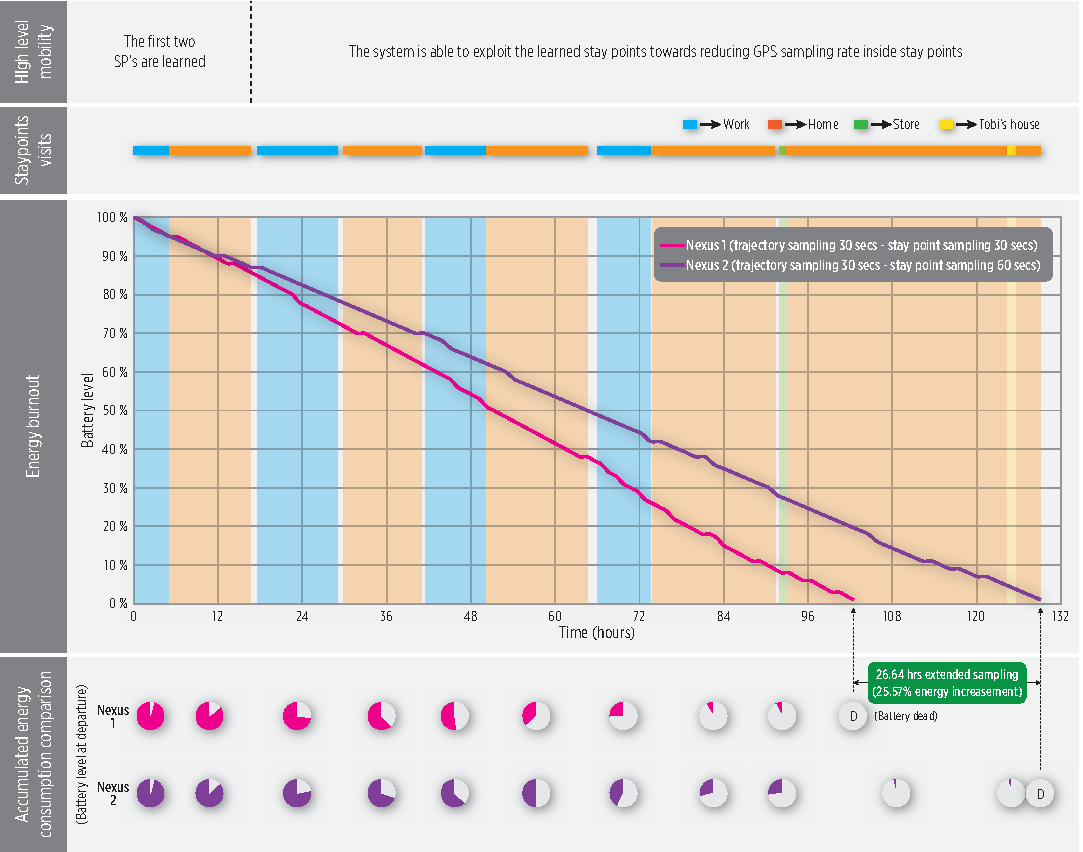
\includegraphics[width=0.8\textwidth]{vectors/energy-results-v2}
%   \captionof{figure}{Energy performance obtained by the CDS along the mobility described by user (trial corresponding to the 30 seconds in trajectory and 60 seconds in stay point sampling).}
%   \par
% }
% \end{frame}

% \begin{frame}[noframenumbering]{Preliminary experimentation}{Energy consumption of fixed-sampling periods: Results}
% \begin{figure}
%   % \includegraphics[width=0.8\textwidth]{vectors/exp-6-map-trj-4-adaptive-sampling-60-sp}
%   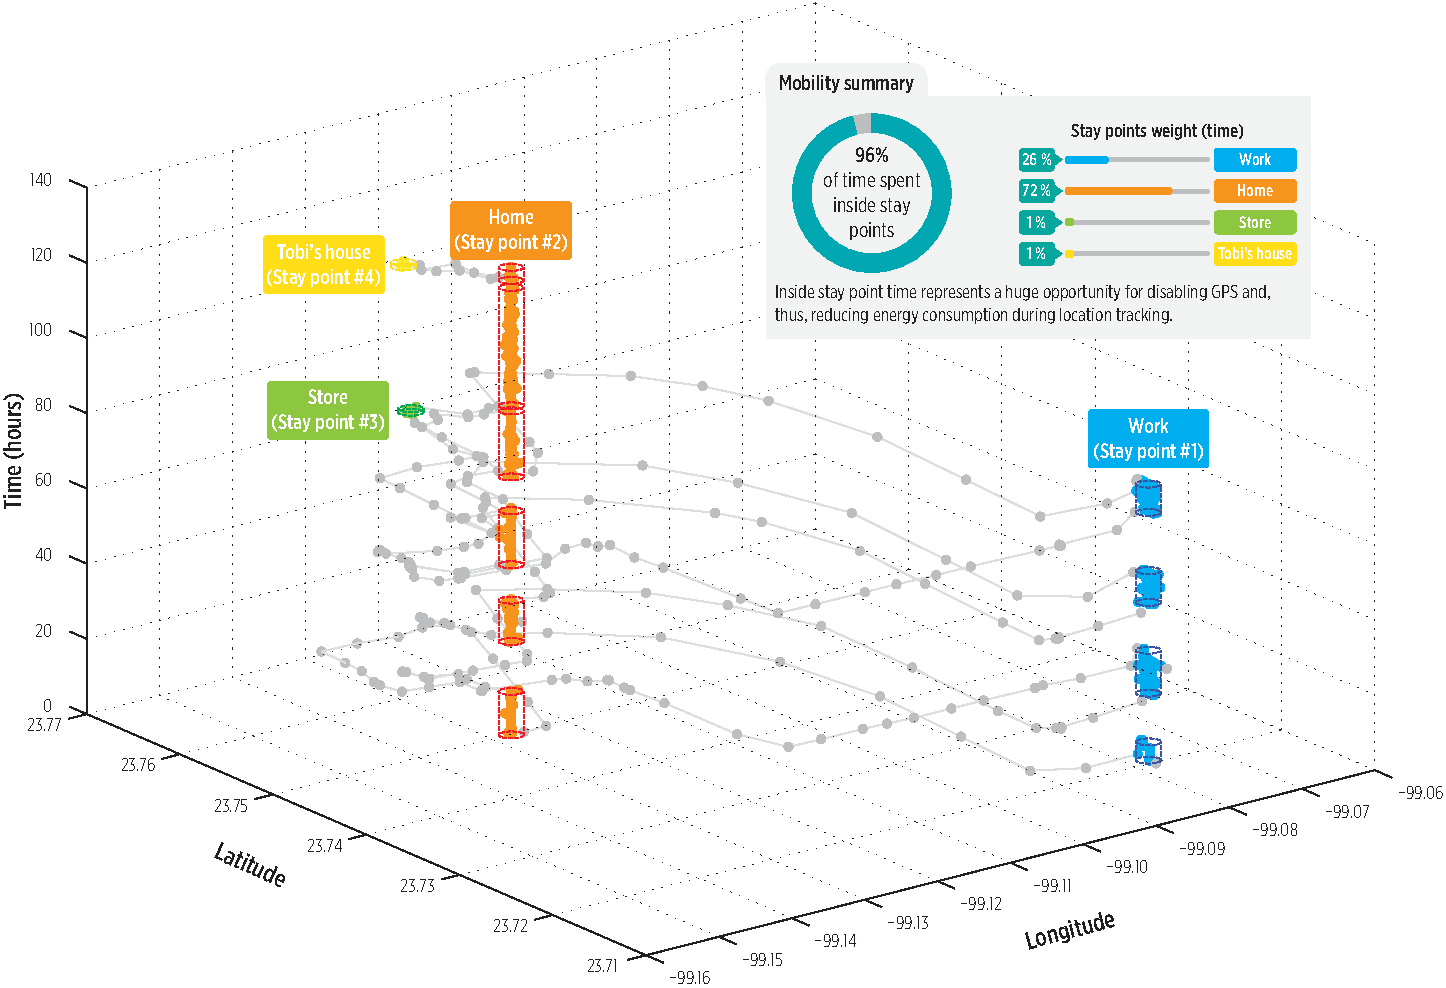
\includegraphics[width=0.85\textwidth]{vectors/stay-points-as-3d-v2}
%   \caption{The stay points and visits identified by the system, as well as the mobility summary obtained from such information (trial corresponding to the 30 seconds in trajectory and 60 seconds in stay point sampling).}
% %  \caption{The information autonomously learned by the STM during the trial corresponding to the 30 seconds in trajectory and 60 seconds in stay point sampling scheme. The height of cylinders corresponds with the stay time during each stay point visit.}
% \end{figure}
% \end{frame}

\end{document}
